\documentclass[10pt]{memoir}
\setstocksize{220mm}{155mm} 	        
\settrimmedsize{220mm}{155mm}{*}	
\settypeblocksize{170mm}{116mm}{*}	
\setlrmargins{18mm}{*}{*}
\setulmargins{*}{*}{1.2}
%\setlength{\headheight}{5pt}%
\checkandfixthelayout[lines]
\linespread{1.16}
\flushbottom

%%% Hyphenation settings
\usepackage[htt]{hyphenat}
\hyphenation{he-lio-trope opos-sum}
\tracingparagraphs=1
%Hyphenation in Devanāgarī of the edition still missing? Probably this needs to be modified in babel-iast package? 

%%% babel
\usepackage[english]{babel}
\usepackage{babel-iast/babel-iast}

\babelfont[iast]{rm}[Renderer=Harfbuzz, Scale=1.3]{AdishilaSan}%AdishilaSan}
\babelfont[english]{rm}{Adobe Text Pro}

%%% more functionality
\PassOptionsToPackage{hyphens}{url}
\usepackage{hyperref}
\usepackage{pdflscape}
\usepackage{cleveref}
\usepackage{url}
\usepackage{cleveref}
\usepackage{microtype}
\usepackage{lineno}

%\usepackage{bigfoot}
%%% more functions
\usepackage[dvipsnames]{xcolor}
%\usepackage[para,perpage]{footmisc}

%%%für den Counter von Kapiteln und Sätzen! 
\newcommand{\uproman}[1]{\uppercase\expandafter{\romannumeral#1}}
\newcommand{\lowroman}[1]{\romannumeral#1\relax}

\makeindex
\newfontfamily\sanskritfont[Script=Devanagari,Mapping=RomDev,Scale=1.1]{Sanskrit2003}
\usepackage{pifont,fourier-orns,lettrine,psvectorian,paralist,enumitem,pdfpages,wrapfig,tabulary,lettrine,longtable}
\setlist[enumerate]{itemsep=0mm}
\usepackage[autostyle]{csquotes}
\usepackage[defaultlines=2,all]{nowidow}
\usepackage{ellipsis,adforn,booktabs,longtable,url,tikz}
\lineskiplimit=-3pt          

\makechapterstyle{IeT}{%
  \chapterstyle{default}
  \renewcommand*{\printchapternonum}{\centering}
  \renewcommand*{\clearforchapter}{\cleartorecto} 
  \aliaspagestyle{chapter}{empty}}
\chapterstyle{IeT}
\setsecnumdepth{none}  \openright  \nouppercaseheads
\settocdepth{subsubsection}

%%%% test better pagebreaks
%\def\fussy{%
%  \emergencystretch\z@
%  \tolerance 200%
%  \hfuzz .1\p@
%  \vfuzz\hfuzz}

%\interfootnotelinepenalty=10000\relax

%\usepackage[maxfloats=256]{morefloats}

%\maxdeadcycles=500

%raggedbottomsectiontrue
%%\checkandfixthelayout


%%%%%%%  biblatex
%\newcommand{\noun}[1]{\textsc{#1}}    %  philosophy-verbose
\usepackage[backend=biber, sorting=nyt, style=verbose]{biblatex} %%%%ORIGINAL TiE
\renewcommand*{\mkbibnamefamily}[1]{\textsc{#1}}


\DeclareFieldFormat{url}{%
  \mkbibacro{URL}\addcolon\space
  \href{#1}{\nolinkurl{\thefield{urlraw}}}}

\DeclareFieldFormat{citeurl}{%
  \href{#1}{\nolinkurl{\thefield{urlraw}}}} 


\DeclareFieldFormat{postnote}{#1}
\renewcommand{\postnotedelim}{, }
\addbibresource{bindu.bib}

%%% ekdosis
\usepackage[teiexport=tidy,parnotes=true]{ekdosis}% =tidy cleans up HTML and XML documents by fixing markup errors and upgrading legacy code to modern standards. parnotes=footnotes below or above critical apparatus

\SetLineation{lineation=page, modulo} %lineation=page sets thenumbering to start afresh at the top of each page. =modulo makes every fifth line numbered. {lineation=page} makes every line numbered! 

\renewcommand{\linenumberfont}{\selectlanguage{english}\footnotesize} %sets language of lines to English

\SetTEIxmlExport{autopar=false} %autopar=falseinstructs ekdosis to ignore blank lines in the.tex sourcefile as markers for paragraph boundaries. As a result, each paragraph of the edition must be found within an environment associated with the xml <p> element

\SetHooks{
  lemmastyle=\bfseries,
  %refnumstyle=\selectlanguage{english}\bfseries,
  refnumstyle=\selectlanguage{english}\color{blue}\bfseries,
  appheight=0.8\textheight,
}

\newif\ifinapparatus
\DeclareApparatus{source}[
%bhook=\inapparatustrue,
lang=english,
notelang=english,
% bhook=\selectlanguage{english},
bhook=\selectlanguage{english}\textbf{Sources:},%
%maxentries=4, 
%ehook=.]
%sep={] },
%nosep,
]

\newif\ifinapparatus
\DeclareApparatus{testium}[
%bhook=\inapparatustrue,
lang=english,
notelang=english,
% bhook=\selectlanguage{english},
bhook=\selectlanguage{english}\textbf{Testimonia:},
%maxentries=4, 
%ehook=.]
%nosep, 
]

% Declare \ifinapparatus and set \inapparatustrue at the beginning of
% the apparatus criticus block. Also set the language.  
\newif\ifinapparatus
  \DeclareApparatus{default}[
  %bhook=\inapparatustrue, 
  lang=english,
  %maxentries=33,
  %bhook=\selectlanguage{english},
  sep = {] },
  delim=\hskip 0.75em,
  rule=\rule{0.7in}{0.4pt},
]

\newif\ifinapparatus
\DeclareApparatus{philcomm}[
%bhook=\inapparatustrue,
lang=english,
notelang=english,
bhook=\selectlanguage{english}\textbf{Philological Commentary:},
%bhook=\selectlanguage{english},
sep={: },
]

\ekdsetup{
showpagebreaks,
spbmk = \textcolor{blue}{spb},
hpbmk = \textcolor{red}{hpb}
}

%\usepackage{fnpos}
%\makeFNmid
%\makeFNbottom
\usepackage[bottom]{footmisc}
%%%%%%%%%%%%%%%%%%%%%%%%%%%
\makeatletter
\def\blfootnote{\gdef\@thefnmark{}\@footnotetext}
\makeatother
%%%%%%%%%%%%%%%%%%%%%%%%%


% Macros and Definitions for the Print of Sigla
\def\acpc#1#2#3{{#1}\rlap{\textrm{\textsuperscript{#3}}}\textsubscript{\textrm{#2}}\space}
\def\sigl#1#2{{{#1}}\textsubscript{\textrm{#2}}}
\def\None{{\sigl{N}{1}}} \def\Noneac{\acpc{N}{1}{ac}\,} \def\Nonepc{\acpc{N}{1}{pc}\,}
\def\Ntwo{{\sigl{N}{2}}} \def\Noneac{\acpc{N}{2}{ac}\,} \def\Nonepc{\acpc{N}{2}{pc}\,}
\def\Done{{\sigl{D}{1}}} \def\Doneac{\acpc{D}{1}{ac}\,} \def\Donepc{\acpc{D}{1}{pc}\,}
\def\Dtwo{{\sigl{D}{2}}} \def\Dtwoac{\acpc{D}{2}{ac}\,} \def\Dtwopc{\acpc{D}{2}{pc}\,}
\def\Uone{{\sigl{U}{1}}} \def\Uoneac{\acpc{U}{1}{ac}\,} \def\Uonepc{\acpc{U}{1}{pc}\,}                 
\def\Utwo{{\sigl{U}{2}}} \def\Utwoac{\acpc{U}{2}{ac}\,} \def\Utwopc{\acpc{U}{2}{pc}\,}

%%%%%%%%%%%%%% Tattvabinduyoga - List of Witnesses   %%%%%%%%%%%%%%%%%%%
\DeclareWitness{ceteri}{\selectlanguage{english}cett.}{ceteri}[]   
\DeclareWitness{E}{\selectlanguage{english}E}{Printed Edition}[]    
\DeclareWitness{P}{\selectlanguage{english}P}{Pune BORI 664}[]  
\DeclareWitness{B}{\selectlanguage{english}B}{Bodleian 485}[]       
\DeclareWitness{N1}{\selectlanguage{english}N\textsubscript{1}}{NGMPP 38/31}[]
\DeclareWitness{N2}{\selectlanguage{english}N\textsubscript{2}}{NGMPP B 38/35}[]
\DeclareWitness{L}{\selectlanguage{english}L}{LALCHAND 5876}[]  
\DeclareWitness{D}{\selectlanguage{english}D}{IGNCA 30019}[] 
%\DeclareWitness{D2}{\selectlanguage{english}D\textsubscript{2}}{IGNCA 30020}[]  
\DeclareWitness{U1}{\selectlanguage{english}U\textsubscript{1}}{SORI 1574}[] 
\DeclareWitness{U2}{\selectlanguage{english}U\textsubscript{2}}{SORI 6082}[]
%%%%%%%%%%%%%% Tattvabinduyoga - Groups of Witnesses   %%%%%%%%%%%%%%%%%%%
\DeclareWitness{X}{\selectlanguage{english}\alpha}{Alpha Group: D,N1,N2,U1}[]
\DeclareWitness{Y}{\selectlanguage{english}\beta}{Beta Group: B,E,L,P,U2}[]
%%%%%%%%%%%%% Testimonia
\DeclareWitness{Ysv}{\selectlanguage{english}Ysv}{Yogasvarodaya}[] %%%add infos!  

%%%%%%%%%%%%%%%%%%%%%%%%%%%%%%%%%%%%%%%%%%%
% Macro for Editing Abbrevs.
\def\om{\textrm{\footnotesize \textit{om.}\ }} %prints om. for omitted in apparatus
\def\korr{\textrm{\footnotesize \textit{em.}\ }} %prints em. for emended in apparatus
\def\conj{\textrm{\footnotesize \textit{conj.}\ }} %prints conj. for conjectured in apparatus

% \supplied{text} EDITORIAL ADDITION -> Within \lem oder \rdg
% \surplus{text} EDITORIAL DELETION -> Within \lem oder \rdg
% \sic{text} CRUX
% \gap{text} LACUNAE -> [reason=??, unit=??, quantity=??, extent=??]


%%%%%%%%%%%%%%%%%%%%%%%%%%%%%%%%%%%%%%%%%%% All macros of this list can be used in 
% Macro for Editing Abbrevs.
\def\eyeskip{\textrm{{ab.\,oc. }}}
\def\aberratio{\textrm{{ab.\,oc. }}}
\def\ad{\textrm{{ad}}}
\def\add{\textrm{{add.\ }}}
\def\ann{\textrm{{ann.\ }}}
\def\ante{\textrm{{ante }}} 
\def\post{\textrm{{post }}}
%\def\ceteri{cett.\,}                   
\def\codd{\textrm{{codd.\ }}}

\def\coni{\textrm{{coni.\ }}}
\def\contin{\textrm{{contin.\ }}}
\def\corr{\textrm{{corr.\ }}}
\def\del{\textrm{{del.\ }}}
\def\dub{\textrm{{ dub.\ }}}

\def\expl{\textrm{{explic.\ }}} 
\def\explica t{\textrm{{explic.\ }}}
\def\fol{\textrm{{fol.\ }}}
\def\foll{\textrm{{foll.\ }}}
\def\gloss{\textrm{{glossa ad }}}
\def\ins{\textrm{{ins.\ }}}      
\def\inseruit{\textrm{{ins.\ }}} 
\def\im{{\kern-.7pt\lower-1ex\hbox{\textrm{\tiny{\emph{i.m.}}}\kern0pt}}} %\textrm{\scriptsize{i.m.\ }}}      
\def\inmargine{{\kern-.7pt\lower-.7ex\hbox{\textrm{\tiny{\emph{i.m.}}}\kern0pt}}}%\textrm{\scriptsize{i.m.\ }}}      
\def\intextu{{\kern-.7pt\lower-.95ex\hbox{\textrm{\tiny{\emph{i.t.}}}\kern0pt}}}%\textrm{\scriptsize{i.t.\ }}}           
\def\indist{\textrm{{indis.\ }}}  
\def\indis{\textrm{{indis.\ }}}
\def\iteravit{\textrm{{iter.\ }}} 
\def\iter{\textrm{{iter.\ }}}
\def\lectio{\textrm{{lect.\ }}}   
\def\lec{\textrm{{lect.\ }}}
\def\leginequit{\textrm{{l.n. }}} 
\def\legn{\textrm{{l.n. }}}
\def\illeg{\textrm{{l.n. }}}

\def\primman{\textrm{{pr.m.}}}
\def\prob{\textrm{{prob.}}}
\def\rep{\textrm{{repetitio }}}
\def\secundamanu{\textrm{\scriptsize{s.m.}}}            \def\secm{{\kern-.6pt\lower-.91ex\hbox{\textrm{\tiny{\emph{s.m.}}}\kern0pt}}}%   \textrm{\scriptsize{s.m.}}}
\def\sequentia{\textrm{{seq.\,inv.\ }}}  
\def\seqinv{\textrm{{seq.\,inv.\ }}}
\def\order{\textrm{{seq.\,inv.\ }}}
\def\supralineam{{\kern-.7pt\lower-.91ex\hbox{\textrm{\tiny{\emph{s.l.}}}\kern0pt}}} %\textrm{\scriptsize{s.l.}}}
\def\interlineam{{\kern-.7pt\lower-.91ex\hbox{\textrm{\tiny{\emph{s.l.}}}\kern0pt}}}   %\textrm{\scriptsize{s.l.}}}
\def\vl{\textrm{v.l.}}   \def\varlec{\textrm{v.l.}} \def\varialectio{\textrm{v.l.}}
\def\vide{\textrm{{cf.\ }}}
\def\cf{\textrm{{cf.\ }}} 
\def\videtur{\textrm{{vid.\,ut}}}
\def\crux{\textup{[\ldots]} }
\def\cruxx{\textup{[\ldots]}}
\def\unm{\textit{unm.}}
%%%%%%%%%%%%%%%%%%%%%%%%%%%%%%%%%%%%

% List of Scholars
\DeclareScholar{ego}{ego}[
forename=Nils Jacob,
surname=Liersch]

% Persons:14\DeclareScholar{ego}{ego}[15forename=Robert,16surname=Alessi]17% Useful shorthands:18\DeclareShorthand{codd}{codd.}{V,I,R,H}19\DeclareShorthand{edd}{edd.}{Lit,Erm,Sm}20\DeclareShorthand{egoscr}{\emph{scripsi}}{ego}

%Useful shorthands:
%\DeclareShorthand{codd}{codd.}{V,I,R,H}
%\DeclareShorthand{edd}{edd.}{Lit,Erm,Sm}
\DeclareShorthand{egoscr}{em.}{ego}
\DeclareShorthand{egoscrconj}{conj.}{ego}
\DeclareShorthand{egomute}{\unskip}{ego}

\usepackage{xparse}

\NewDocumentEnvironment{tlg}{O{}O{}}{\setlength{\leftskip}{0pt}\vspace{-1ex}\begin{quotation}}{\hfill #1\ \vspace{-1ex}\end{quotation}\vspace{-1ex}} %verse environment
%\NewDocumentEnvironment{tlg}{O{}O{}}{\begin{verse}}{॥#1\hskip-4pt ॥\\ \end{verse}}
\NewDocumentCommand{\tl}{m}{{\selectlanguage{iast} #1}}

\NewDocumentCommand{\extra}{m}{{\textcolor{gray}{#1}}} %command for additions to U2
\NewDocumentCommand{\crazy}{m}{{\textcolor{red}{#1}}} %totally corrupted passage
\NewDocumentCommand{\coro}{m}{{\textcolor{violet}{#1}}} %colour for sentence counter! 

\NewDocumentEnvironment{prose}{O{}}{\begin{otherlanguage}{iast}}{\end{otherlanguage}}
% \NewDocumentEnvironment{padd}{O{}}{\begin{otherlanguage}{iast}}{\end{otherlanguage}}
\NewDocumentEnvironment{tlate}{O{}}
%\NewDocumentEnvironment{tadd}{O{}}

%Define two commands: \skp ("sanskrit plus"), to be ignored by TeX in
%the edition text, but processed in the TEI output. Conversely, \skm
%("sanskrit minus") is to be processed in the edition text, but
%ignored if found in the apparatus criticus and in the TEI output:

\NewDocumentCommand{\skp}{m}{}
\TeXtoTEIPat{\skp {#1}}{#1}

%\NewDocumentCommand{\skpp}{m}{}
%\TeXtoTEIPat{\skpp {#1}}{#1}

\NewDocumentCommand{\skm}{m}{\unless\ifinapparatus#1-\fi}
\TeXtoTEIPat{\skm {#1}}{}

% \NewDocumentCommand{\dd}{}{/\hskip-4pt/}
\NewDocumentCommand{\dd}{}{\mbox{/\hskip-4pt/}}
\TeXtoTEIPat{\dd {}}{//}


%%% modify environments and commands
%%% TEI mapping
\TeXtoTEIPat{\begin {tlg}}{<lg>} %lg=(Group of verse (s)) contains one or more verses or lines of verse that together form a formal unit (e.g. stanza, chorus).
\TeXtoTEIPat{\end {tlg}}{</lg>}

\TeXtoTEIPat{\begin {prose}}{<p>}
\TeXtoTEIPat{\end {prose}}{</p>}

\TeXtoTEIPat{\begin {tlate}}{<p>}
\TeXtoTEIPat{\end {tlate}}{</p>}

\TeXtoTEIPat{\\}{}
\TeXtoTEIPat{\linebreak}{<br/>}
\TeXtoTEIPat{\noindent}{}
%\TeXtoTEI{tl}{l}
\TeXtoTEI{emph}{hi}
\TeXtoTEI{bigskip}{}
\TeXtoTEI{None}{N1}
\TeXtoTEI{Ntwo}{N2}
\TeXtoTEI{Done}{D1}
\TeXtoTEI{Dtwo}{D2}
\TeXtoTEI{Uone}{U1}
\TeXtoTEI{Utwo}{U2}
%\TeXtoTEIPat{/}{ |}
%\TeXtoTEI{//}{ ||}
\TeXtoTEIPat{\korr}{em. }
\TeXtoTEIPat{\conj}{conj.}
\TeXtoTEIPat{\om}{om.}
\TeXtoTEIPat{english}{}
\TeXtoTEIPat{\hskip}{}
\TeXtoTEIPat{\hskip-4pt}{}
\TeXtoTEIPat{\hskip-2pt}{}
\TeXtoTEIPat{-}{ }
\TeXtoTEIPat{4pt}{}
\TeXtoTEIPat{2pt}{}
\TeXtoTEIPat{\textcolor {#1}{#2}}{<hi rend="#1">#2</hi>} 

% Nullify \selectlanguage in TEI as it has been used in
% \DeclareWitness but should be ignored in TEI.
\TeXtoTEI{selectlanguage}{}



\FormatDiv{1}{\begin{center}\Large}{\end{center}}
\FormatDiv{2}{\begin{center}\small}{\end{center}}
\FormatDiv{3}{\bfseries}{.}
\title{Yogatattvabindu of Rāmacandra\\ A Critical Edition and Annotated Translation}
\date{\today}

\parindent=15pt
\begin{document}

% Zitiermöglichkeiten:
%\footcite[See][p.\,1]{goldstein01:_tibet_englis_diction_moder_tibet}
%\footnote{\cite{goldstein01:_tibet_englis_diction_moder_tibet}.}

\frontmatter
\thispagestyle{empty}
\begin{center}
  {\Large \emph{The Yogatattvabindu}}\\[3mm]
\end{center}



\newpage

\

\thispagestyle{empty}



\normalsize


\newpage


\begin{center}
\thispagestyle{empty}

\

\vskip 2mm

\begin{otherlanguage}{iast}
\LARGE \sanskritfont{Yogatattvabindu}
\end{otherlanguage}

\vskip .4cm

\Huge Yogatattvabindu \\[7mm]
\Large Critical Edition\\
with annotated Translation


\large

\vspace{3cm}

Von

Nils Jacob Liersch
\small
\vfill

\vfill

Indica et Tibetica Verlag \\ % $\cdot$ 
Marburg 2024

\vskip 6mm

\end{center}

\newpage
\newpage \ \thispagestyle{empty}
\small  \

\noindent

\
\vfill


\small
\noindent \textbf{Bibliographische Information Der Deutschen Bibliothek}

\noindent
Die Deutsche Bibliothek verzeichnet diese Publikation in der Deutschen Nationalbibliographie;
detaillierte bibliographische Informationen sind im Internet über http://dnb.ddb.de abrufbar.

\noindent
\textbf{Bibliographic information published by Die Deutschen Bibliothek}

\noindent
Die Deutsche Bibliothek lists this publication in the Deutsche Nationalbibliographie; detailed
bibliographic data is available in the Internet at http://dnb.ddb.de.  


\vskip 1cm

\noindent
\copyright\ Indica et Tibetica Verlag, Marburg 2024

\medskip

\noindent
Alle Rechte vorbehalten / All rights reserved

\medskip

\noindent
Ohne ausdrückliche Genehmigung des Verlages ist es nicht gestattet, das Werk oder einzelne Teile
daraus nachzudrucken, zu vervielfältigen oder auf Datenträger zu speichern.

\smallskip

\noindent
Apart from any fair dealing for the purpose of private study, research, criticism or review, no
part of this book may be reproduced or translated in any form, by print, photo form, microfilm, or
any other means without written permission. Enquiries should be made to the publishers.

\bigskip

\noindent
Satz: \ \ Nils Jacob Liersch \\
Herstellung: \ \ BoD – Books on Demand GmbH, Norderstedt  \\

\bigskip

\noindent
%\ISBN     

\normalsize

\newpage

%\maketitle
\clearpage
\tableofcontents
\addtocounter{page}{-1}
\thispagestyle{empty}
\clearpage


\mainmatter

\chapter{Conventions in the Critical Apparatus}
\section{Sigla in the Critical Apparatus}

\begin{itemize}
\item E : Printed Edition
\item P : Pune BORI 664
\item L : Lalchand Research Library LRL5876
\item B : Bodleian Oxford D 4587
‚\item \None : NGMPP B 38-31
\item \Ntwo : NGMPP B 38-35 / A 1327-14
\item \Done : IGNCA 30019
\item \Uone : SORI 1574
\item \Utwo: SORI 6082
\end{itemize}

\chapter{Critical Edition \& Annotated Translation}
\cleardoublepage
\begin{alignment}[
  texts=edition[class="edition"];
  translation[class="translation"],
  ]
  \begin{edition}
    \ekddiv{
      head={[\uproman{22}. \textbf{svabhāvabhedam}]},
      type=section,
      depth=2, 
      n=XXII
    }
    \xmlhead[h22]{[XXII. svabhāvabhedam]}
    \begin{prose}[p22_01]
      \label{svabhava1}
            \noindent
%------------------------------
%idānīṃ tasya---bhedaḥ    kathyate/   \E
%idānīṃ svabhāvabhedaḥ kathyate    \P
%idānī  svābhāvabhedaḥ kathyate//  \B
%idānīṃ svābhāvabhedaḥ kathyate//  \L
%idānīṃ svabhāvabhedaṃ kathyate//  \N1
%idānīṃ svabhāvabhedaṃ kathyate//  \D
%idānīṃ svabhāvabheda  kathyate//  \N2
%idānīṃ svabhāvabhedāḥ kathyate    \U1
%idānīṃ svabhāvabhedaḥ kathyate//  \U2
%------------------------------
%Now, the division of the inherent being is described. 
%------------------------------  
\note[type=source, labelb=_143i, labele=_145e, nosep]{cf. YSv (PT p. 836): svabhāvabhedam etat śṛṇu devi prayatnataḥ | yac chrutvā sarvabodhaḥ syāt muktidaḥ siddhivāñchitaḥ | ātmano vā pṛthivyādyāḥ svabhāvaḥ kiñcid ucyate |}
\linelabel{_143i}
\app{\lem[wit={ceteri}]{idānīṃ}
  \rdg[wit={B}]{idānī}}
\app{\lem[wit={ceteri},alt={svabhāva°}]{svabhāva}
  \rdg[wit={B,L}]{svābhāva°}
  \rdg[wit={E}]{tasya}
}\app{\lem[wit={D,N1},alt={°bhedaṃ}]{bhedaṃ}
  \rdg[wit={N2}]{°bheda}
  \rdg[wit={ceteri}]{°bhedaḥ}}
kathyate/
%------------------------------  
%yathā vaṭabījam/ vaṭarūpeṇa pariṇataṃ    sat    daśadhā    bhedaṃ svabhāvata eva prāpnoti/  \E %%%[P.27]
%yathā vaṭabījaṃ  vaṭarūpeṇa pariṇāte     sat    dṛśadhā    bhedaṃ svabhāvata eva prāpnoti   \P
%yathā vaṭabījena rūpeṇa     pariṇamate/  śata   daśadhā    bhedaṃ svābhāva   eva prāpnotī// \B
%yathā vaṭabījena rūpeṇa     pariṇamate   śata   daśadhā    bhedaṃ svābhāva   eva prāpnotī// \L
%yathā vaṭabījaṃ  vaṭarūpeṇa pariṇataṃ//  satṛ   daśadhā    bhedaṃ svabhāvata eva prāpnoti/  \N1
%yathā vaṭabījaṃ  vaṭarūpeṇa pariṇataṃ/   sa     daśadhā    bhedaṃ svabhāvata eva prāpnoti// \D
%yathā vathabījaṃ vaṭarūpeṇa pariṇataṃ/   sa tu  daśadhā    bhedaṃ svabhāvata eva prāpnoti/  \N2
%yathā vaṭabījaṃ  vaṭarūpeṇa pariṇataṃ    sa tat daśadhā    bhedaṃ svabhāvata eva prāpnotī   \U1
%yathā vaṭabīja---vaṭarūpeṇa pariṇamate// sa     dasat                            prāpnoti// \U2
%------------------------------
%Just as the seed of the banyan tree ripens into the shape of the banyan tree, [and] because of its own inherent being develops such a tenfold division. [Namely]:
%------------------------------
yathā
\app{\lem[wit={ceteri},alt={vaṭa°}]{vaṭa}
  \rdg[wit={N2}]{vatha°}
}\app{\lem[wit={D,P,N1,N2,U1},alt={°bījaṃ}]{bījaṃ}
        \rdg[wit={E}]{°bījam}
        \rdg[wit={U2}]{°bīja°}
        \rdg[wit={B,L}]{°bījena}}
      \app{\lem[wit={ceteri}]{vaṭarūpeṇa}
        \rdg[wit={B,L}]{rūpeṇa}}
      \app{\lem[wit={B,L,U2}]{pariṇamate}
        \rdg[wit={P}]{pariṇāte}
        \rdg[wit={X,E}]{pariṇataṃ}}
      \app{\lem[type=emendation, resp=egoscr, alt={sa tad}]{sa ta\skp{d-da}}
        \rdg[wit={U1},alt={sa tat}]{sa tat}
        \rdg[wit={N2}]{sa tu}
        \rdg[wit={N1}]{satṛ}
        \rdg[wit={E,P}]{sat}
        \rdg[wit={B,L}]{śata}
        \rdg[wit={D,U2}]{sa}
      }\app{\lem[wit={ceteri},alt={daśadhā}]{\skm{d-da}śadhā}
        \rdg[wit={P}]{dṛśadhā}
        \rdg[wit={U2}]{dasat}}
      \app{\lem[wit={ceteri}]{bhedaṃ}
        \rdg[wit={U2}]{\om}}
      \app{\lem[wit={ceteri}]{svabhāvata}
        \rdg[wit={B,L}]{svabhāva}
        \rdg[wit={U2}]{\om}}
      \app{\lem[wit={ceteri}]{eva}
        \rdg[wit={U2}]{\om}}
      \app{\lem[wit={ceteri}]{prāpnoti}
        \rdg[wit={B,L,U1}]{prāpnotī}}/
%------------------------------ %%%%STEMMA POINT!!!!
%mūlāṃkura---tvagdaṇḍaśākhā--kalikāpallavapuṣpaphalasnehā                  iti daśabhedān    prāpnoti// \E
%mūla aṃkura-tvakdaṃdaśākhā----kilpikāpallavā puṣpaphalasneha              iti daśabhedān    prāpnotīti \P  %%%7642.jpg
%mūlaṃ aṃkuratvakdaṃdaśākhā----kilakālapallavā// vistāroyaṃ svābhāvataḥ    iti daśabhedān    prāpnoti// \B DSCN7160 Z. 4
%mūlaṃ aṃkuratvakdaṃdaśākhā----kilāpallavā// vistāroyaṃ svābhāvataḥ//      iti daśabhedān    prāpnoti... \L
%mūlāṃ aṃkuratvakdaṃḍaśākhāṃ kalikāpallavapuṣpaphalasneha//                iti bhedo daśadhā prāpnoti// \N1
%mūlāṃkura---tvakdaṇdaśākhāṃ kalikāpallavapuṣpaphalasnehaṃ                 iti bhedo daśadhā prāpnoti// \D
%mūlāṃkura---tvakdaṇdaśākhāṃ kalikāpallavapuṣpaphalasneha/                 iti bhedo daśadhā prāpnoti// \N2
%mūlāṃaṃkura-tvakdaṇdaśākhā--kalikāpallavapuṣpaphalasneha                  iti bhedo daśadhā prāpnoti \U1
%\om                                                                                \U2
%------------------------------
%"Wurzel, Spross, Rinde, Ast, Zweig, Knospe, die sich entfaltende Blüte, Blüte, Frucht und Nektar." Die Auftheilung erreicht [diese] zehn Teile. 
%------------------------------
%"Root, shoot, bark, branch, twig, bud, the unfolding flower, flower, fruit and nectar." The division reaches [those] ten parts.
%------------------------------
\app{\lem[wit={E}]{mūlāṅkuratvagdaṇḍaśākhākalikāpallavapuṣpaphalasnehā}
          \rdg[wit={P}]{mūla aṃkuratvakdaṃdaśākhākilpikāpallavā puṣpaphalasneha}
          \rdg[wit={B}]{mūlaṃ aṃkuratvakdaṃdaśākhākilakālapallavā || vistāroyaṃ svābhāvataḥ}
          \rdg[wit={L}]{mūlaṃ aṃkuratvakdaṃdaśākhākilāpallavā || vistāroyaṃ svābhāvataḥ ||}
          \rdg[wit={N1}]{mūlāṃ aṃkuratvakdaṃḍaśākhāṃ kalikāpallavapuṣpaphalasneha ||}
          \rdg[wit={N2}]{mūlāṃkuratvakdaṇdaśākhāṃ kalikāpallavapuṣpaphalasneha|}
          \rdg[wit={D}]{mūlāṃkuratvakdaṇdaśākhāṃ kalikāpallavapuṣpaphalasnehaṃ}
          \rdg[wit={U1}]{mūlāṃ aṃkuratvakdaṇdaśākhākalikāpallavapuṣpaphalasneha}
          \rdg[wit={U2}]{\om}}
        \app{\lem[wit={ceteri}]{iti}
          \rdg[wit={U2}]{\om}}
        \app{\lem[wit={B,E,L,P}]{daśabhedān}
          \rdg[wit={X}]{bhedo daśadhā}
          \rdg[wit={U2}]{\om}}
        \app{\lem[wit={ceteri}]{prāpnoti}
          \rdg[wit={P}]{prāpnotīti}
          \rdg[wit={U2}]{\om}}/
%------------------------------
%yathā nirmalo  nirvikāraḥ niraṃjana   eka  etādṛśa  ātmā svabhāvād eva/ pṛthivyaptejovāyvākāśamanobuddhimāyāvikārarūpabhedān    prāpnoti/ \E
%tathā nirmalaḥ nirvikāraḥ niraṃjanaḥ  eka  etādṛśa  ātmasvabhāvād eva   pṛthvyetetejo vādvyākāśamanobuddhimāyāvikārarūpabhedāt  prāpnoti \P
%tathā nirmalo  nirvikāraḥ niraṃjanaḥ  eka  etādṛśa  ātmasvabhāvād eva   pṛthvyāpatejovādvyākāśamanobuddhimāyāvikārarūpabhedāna  prāpnoti// \B
%tathā nirmalo  nirvikāraḥ niraṃjanaḥ/ eka  etādṛśa  ātmasvabhāvād eva   pṛthvyāpatejovāybākāśamanobuddhimāyāvikārarūpābhedāna   prāpnoti  \L
%tathā nirmalaḥ nirvikāraḥ niraṃjanaḥ  ekaḥ etādṛśaḥ ātmasvabhāvād eva   pṛthvyāpatejovāybākāśamanobuddhimāyāvikārarūpābhedān    prāpnoti/ \N1
%tathā nirmalaḥ nirvikāraḥ niraṃjanaḥ  eka  etādṛśaḥ ātmasvabhāvād eva   pṛthvīpate/ jīvīkāśamanobuddhir māyāvikārarūpabhedāt    prāpnoti \D
%tathā nirmalaḥ nirvikāraḥ niraṃjanaḥ  ekaḥ etādṛśaḥ ātmasvabhāvād eva   pṛthvīpate/ jīvīkāśamanobuddhir māyāvikārarūpabhedāt    prāpnoti/ \N2
%tathā nirmalaḥ nirvikāraḥ niraṃjanaḥ  ekaḥ etādṛśaḥ ātmascabhāvād eva   pṛthakte jīvāyuvākāśamanobuddhir māyāyāvikārarūpabhedāt prāpnoti \U1 %%%275.jpg
%yathā nirmalaḥ nirvikāraḥ niraṃjanaḥ  eka  etādṛśa  ātmasvabhāvād eva// pṛthvyaptejovāyyākāśa// manobuddhimayāvikārarūpabhedān  prāpnoti/ \U2
%------------------------------
%In dieser Weise erreicht auch das reine, unveränderliche, makellose, eine solche [Auftheilung] eben aufgrund der inhärenten Natur des Selbst. [Nämlich] die Aufteilung "Erde, Wasser, Feuer, Wind, Raum, Geist, Intellektekt, Illusion, Umwandlungen und Gestalt".
%------------------------------
%In this way, the pure, unchanging, unblemished, attains such [a division] precisely, because of the inherent being of the self. [Namely] the division: "Earth, water, fire, wind, space, mind, intellect, illusion, transformations and form".
%------------------------------
        \app{\lem[wit={ceteri}]{tathā}
            \rdg[wit={E,U2}]{yathā}}
          \app{\lem[wit={B,E,L}]{nirmalo}
            \rdg[wit={X,P,U2}]{nirmalaḥ}}
          nirvikāraḥ
          \app{\lem[wit={E}, alt={nirañjana}]{nirañjana}
            \rdg[wit={ceteri}]{niraṃjanaḥ}}
          \app{\lem[wit={ceteri}]{eka}
            \rdg[wit={N1,N2,U1}]{ekaḥ}}
          \app{\lem[wit={E}]{etādṛśa}
            \rdg[wit={N1,N2,U1}]{etādṛśaḥ}}
          \app{\lem[wit={ceteri}, alt={ātmasvabhāvād}]{ātmasvabhāvā\skp{d-e}}
            \rdg[wit={E}]{ātmā svabhāvād}
          }\skm{d-e}va
          \app{\lem[wit={B,L}, alt={pṛthvyāpatejovāyvākāśamanobuddhimāyāvikārarūpabhedān}]{pṛthvyāpatejovāyvākāśamanobuddhimāyāvikārarūpabhedā\skp{n-prā}}
            \rdg[wit={N1}]{pṛthvyāpatejovāyvākāśamanobuddhimāyāvikārarūpābhedān}
            \rdg[wit={E}]{pṛthivyapāpatejovāybākāśamanobuddhimāyāvikārarūpābhedān}
            \rdg[wit={P}]{pṛthvyetetejovādvyākāśamanobuddhimāyāvikārarūpābhedān}
            \rdg[wit={D,N2}]{pṛthvīpate | jīvīkāśamanobuddhir māyāvikārarūpabhedāt}
            \rdg[wit={U1}]{pṛthakte jīvāyuvākāśamanobuddhir māyāyāvikārarūpabhedāt}
            \rdg[wit={U2}]{pṛthvyaptejovāyyākāśa || manobuddhimayāvikārarūpabhedā}
          }\skm{n-prā}pnoti/
%------------------------------
%jñānayogaprabhāvād     eka eva  ātmā iti niścayo bhavati// \E
%jñānayogaḥ prabhāvād   eka eka  ātmā iti niścayo bhavati \P
%jñānayogaḥ// prabhāvād eka eka  ātmā iti niścayā bhavatī// \B
%jñānayogaḥ// prabhāvād eka eka  ātmā iti niścayo bhavati// \L
%jñānayogaprabhāvāt     eka eva  ātmā iti niścayo bhavati// \N1
%jñānayogaprabhāvāt     eka eva  ātmā iti niścayo bhavati// \D
%jñānayogaprabhāvāt     eka eva  ātmā iti niścayo bhavati// \N2
%jñānayogaprabhāvāt tu  eka yeva ātmā iti niścayo bhavati \U1
%jñānayogaprabhāvād     eka eva  ātmā iti niścayo bhavati// \U2
%------------------------------
%Because of the power of Jñānayoga, there arises the conviction that "the self is truly one".  
%------------------------------
\app{\lem[wit={E,U2}, alt={jñānayogaprabhāvād}]{jñānayogaprabhāvā\skp{d-e}}
  \rdg[wit={X}]{jñānayogabhavāt}
  \rdg[wit={B,L}]{jñānayogaḥ || prabhāvād°}
  \rdg[wit={P}]{jñānayogaḥ prabhāvād}
}\skm{d-e}ka
\app{\lem[wit={ceteri}]{eva}
  \rdg[wit={B,L,P}]{eka}
  \rdg[wit={U1}]{yeva}}
ātmā iti niścayo bhavati/
    \end{prose}
  \end{edition}
  \begin{translation}
   \ekddiv{
   head={[\uproman{22}. \textbf{Division of the Inherent Being}]},
   type=section,
   depth=2, 
   n=XXII.1 
 }
 \xmlhead[h22]{[XXII. Division of the Inherent Being]}
        \begin{tlate}[p22_01]
            \noindent
   Now, the nature of the self and it's distinction\footnote{One comes across the term \textit{svabhāvabheda} in philosophical systems to signify the division or distinction of essential natures. For a Buddhist example, see \citeauthor{balcerowicz2011dharmakirti} (2011: 6 ff.). In some Nyāya texts, the term is picked up to refer to different essential properties of the self, cf., i.e. \citeauthor{ogawa2023perception} (2023: 162). In the \textit{Netratantantra}, the term \textit{bhāvabheda} occurs frequently in a similar sense as in this passage of the \textit{Yogatattvabindu}. For example cf. \textit{Netratantra} 16.20-21 (\textit{bhaviṣyanti mahādevi kaliḥ kaṣṭataro yataḥ} | \textit{tadarthaṃ paramārtho 'yaṃ mayā te prakaṭīkṛtaḥ} | \textit{paramārthaḥ paratvena mṛtyujit sarvatomukhaḥ} | \textit{bhāvabhedena yaṣṭav yo mokṣasiddhim abhīpsatā} |). Here, however, the context is unphilosophical and specifically intended to signify the phenomenological distinction of the self.} is described. Just as the seed of the banyan tree transforms into the shape of the banyan tree - just so, due to its nature it attains a tenfold distinction, `Root, shoot, bark, branch, twig, bud, the unfolding flower, flower, fruit and resin' are the ten distinctions [it] attains. In the same way, the pure, unchanging, immaculate one attains as such precisely because of the nature of the self - [namely], the divisions of earth, water, fire, wind, space, mind, intellect, illusion, transformations, and form.\footnote{Rāmacandra’s tenfold taxonomy of \textit{tattva}s appears inconsistent. Here, besides the stable list of the five gross elements, \textit{ahaṃkāra} is replaced with \textit{rūpa} and the order of the other elements is changed. None of the tenfold \textit{tattva}-systems known to me equal Rāmacandra's systems exactly. Taxonomies of \textit{tattva}s like \citetitle{bhagavadgita} 7.4 in which Kṛṣṇa presents a list of eight divisions of \textit{prakṛti} are almost identical (\textit{bhūmir āpo 'nalo vāyuḥ khaṃ mano buddhir eva cha} | \textit{ahankāra itīyaṃ me bhinnā prakṛitir aṣhṭadhā} ||7.4||). "Earth, water, fire, air, space, mind, intellect, and ego - these are the eight divisions of the original nature." In this list, we find most of the elements of Rāmacandra's list, except terms like \textit{māyā}, \textit{vikāra} or \textit{rūpa}. The description of \textit{kuṇḍalinī} in \citetitle{yajnavalkya} 4.21 picks up this system. Another system of ten \textit{tattva}s appears in \textit{Uttarasūtra} 1.9 - 1.13 of the \citetitle{nishvasa2015} in which the tenfold nature of Sadāśiva is homologised with the \textit{mantra}. Here the following list is given: \textit{prakṛti}, \textit{puruṣa}, \textit{niyati}, \textit{kāla}, \textit{māyātattva}, \textit{vidyā}, \textit{Īśvara}, \textit{Sadāśiva}, \textit{dehavyāpin} and \textit{Śakti}, cf. \citeauthor[2016: 83-84]{goodall2016}. There is no similarity between the two tenfold \textit{tattva}-systems. However, since Rājayoga is rooted in ancient Śaivsim (see \citeauthor{birch2019saiva} 2019), and Rāmacandra usually tends to present simplified and transsectarian systems, the choice of a tenfold \textit{tattva}-system might be a remnant of those ancient systems.} Because of the power of Jñānayoga, the conviction arises that `the self is only one'. 
            \flushpage 
            \end{tlate}
  \end{translation}
\end{alignment}
\pagebreak %after pp. 45-46
%%%%%%%%%%%%%%%%%%%%%%%%%%%%%%%%%%%%%%%%%%
%%%%%%%%%%%%%%%%%%%%%%%%%%%%%%%%%%%%%%%%%%
%%%%%%%%PAGEBREAK%%%%%%%PAGEBREAK%%%%%%%%%
%%%%%%%%%%%%%%%%%%%%%%%%%%%%%%%%%%%%%%%%%%
%%%%%%%%%%%%%%%%PAGEBREAK%%%%%%%%%%%%%%%%%
%%%%%%%%%%%%%%%%%%%%%%%%%%%%%%%%%%%%%%%%%%
%%%%%%%%PAGEBREAK%%%%%%%PAGEBREAK%%%%%%%%%
%%%%%%%%%%%%%%%%%%%%%%%%%%%%%%%%%%%%%%%%%%
%%%%%%%%%%%%%%%%%%%%%%%%%%%%%%%%%%%%%%%%%%
%%%%%%%%%%%%%%%%%%%%%%%%%%%%%%%%%%%%%%%%%%
%%%%%%%%%%%%%%%%%%%%%%%%%%%%%%%%%%%%%%%%%%
%%%%%%%%PAGEBREAK%%%%%%%PAGEBREAK%%%%%%%%%
%%%%%%%%%%%%%%%%%%%%%%%%%%%%%%%%%%%%%%%%%%
%%%%%%%%%%%%%%%%PAGEBREAK%%%%%%%%%%%%%%%%%
%%%%%%%%%%%%%%%%%%%%%%%%%%%%%%%%%%%%%%%%%%
%%%%%%%%PAGEBREAK%%%%%%%PAGEBREAK%%%%%%%%%
%%%%%%%%%%%%%%%%%%%%%%%%%%%%%%%%%%%%%%%%%%
%%%%%%%%%%%%%%%%%%%%%%%%%%%%%%%%%%%%%%%%%%
%%%%%%%%%%%%%%%%%%%%%%%%%%%%%%%%%%%%%%%%%%
%%%%%%%%%%%%%%%%%%%%%%%%%%%%%%%%%%%%%%%%%%
%%%%%%%%PAGEBREAK%%%%%%%PAGEBREAK%%%%%%%%%
%%%%%%%%%%%%%%%%%%%%%%%%%%%%%%%%%%%%%%%%%%
%%%%%%%%%%%%%%%%PAGEBREAK%%%%%%%%%%%%%%%%%
%%%%%%%%%%%%%%%%%%%%%%%%%%%%%%%%%%%%%%%%%%
%%%%%%%%PAGEBREAK%%%%%%%PAGEBREAK%%%%%%%%%
%%%%%%%%%%%%%%%%%%%%%%%%%%%%%%%%%%%%%%%%%%
%%%%%%%%%%%%%%%%%%%%%%%%%%%%%%%%%%%%%%%%%%
\begin{alignment}[
  texts=edition[class="edition"];
  translation[class="translation"],
  ]
  \begin{edition}
    \begin{prose}[p22_02]
       \label{svabhava2}
       \noindent
%------------------------------
%yathaikaiva   pṛthvī  kvacit komalarūpā                                                   kvacit parimalarūparahitā kvacit suvarṇarūpā   kvacid raupyarūpā    \E %%%p.28 
%yathā ekaika  pṛthvī  kvacit komalarūpā                                                                                                                       \P   
%yathā ekaika  pṛthvī  kvacit komalarūpā// kvacit manohararūpā//  kvacit parimalarūpayuktā// kvacit parimalarohitā// kvacit suvarṇarūpa                        \B
%yathā ekaika  pṛthvī  kvacit komalarūpā   kvacit manohararūpāḥ// kvacit parimalarūpayuktā// kvacit parimalarahitā// kvacit suvarṇarūpā                        \L
%yathā ekaiva  pṛthivī kvacit komalarūpa/  kvacit manoharā/       kvacit parimalarūpāyuktā// kvacit parimalarahitā/  kvacit suvarṇarūpā/  kvacit rūpyarūpā/    \N1
%yathā ekaiva  pṛthivī kvacit komalarūpa   kvacit manoharā//      kvacit parimalarūpāyuktā/  kvacit parimalarohitā   kvacit suvarṇarūpa// kvacit rūpyarūpa//   \D
%yathā ekaṃ ca pṛthivī kvacit komalarūpa   kvacit manoha?rā       kvacit parimalarūpāyuktaḥ/ kvacit parimalarohitā   kvacit suvarṇarūpā   kvacit rūpyarūpa     \N2
%yathā ekai ca pṛthivī kvacit                                                                                              khavarṇakupā   kvacit rūpyarūpā     \U1
%yathā ekaika  pṛthvī  kvacit komalarūpā// kvacit manohararūpa//  kvacit parimalarūpāyuktā/  kvacit parimalarohitā// kvacit suvarṇarūpā// kvacit rajatarūpā//  \U2
%------------------------------
%As some particular soil (\textit{ekaika}) sometimes appears soft, sometimes appears beautiful, sometimes fragrant, sometimes unscented, sometimes golden, sometimes silver,... 
%------------------------------
\note[type=source, labelb=_143i, labele=_144ie, nosep]{cf. YSv (PT p. 836): ātmaiva pṛthivī dhātrī komalā ca kvacid dṛḍhā | kvacin manoharā sā ca vimalā ca malāmalā | durgandhā ca sugandhā ca nirgandhā gandhamohinī | svarṇarūpā dhāturūpā citrā ratnamayī parā | kvacit śvetā kvacid raktā kvacit pītā ca kṛṣṇalā | ūrvarā ūrvarā sā tu viṣāmṛtamayī sadā |}
\linelabel{_143i}
\app{\lem[type=emendation, resp=egoscr]{yathaikaikaḥ}
  \rdg[wit={E}]{yathaikaiva}
  \rdg[wit={B,L,P,U2}]{yathā ekaika}
  \rdg[wit={D,N1}]{yathā ekaiva}
  \rdg[wit={N2}]{yathā ekaṃ ca}
  \rdg[wit={U1}]{yathā ekai ca}}
\app{\lem[wit={Y}]{pṛthvī}
  \rdg[wit={X}]{pṛthivī}}
kvacit-komala\app{\lem[wit={Y},alt={°rūpā}]{rūpā}
  \rdg[wit={X}]{°rūpa}}\dd{}
%\note[type=philcomm, labelb=145a, labele=_145e, lem={kvacit manohararūpā \ldots kvacit pītā}]{Section is omitted in \getsiglum{P}.}
\app{\lem[wit={ceteri}, alt={kvacit}]{kvaci\skp{t-ma}}
  \rdg[wit={E,P,U1}]{\om}
}\app{\lem[wit={B}, alt={manohararūpā}]{\skm{t-ma}nohararūpā}
  \rdg[wit={L}]{manohararūpāḥ}
  \rdg[wit={U2}]{manohararūpa}
  \rdg[wit={D,N1,N2}]{manoharā}
  \rdg[wit={E,P,U1}]{\om}}\dd{}
\app{\lem[wit={ceteri}, alt={kvacit}]{kvaci\skp{t-pa}}
  \rdg[wit={E,P,U1}]{\om}
}\app{\lem[wit={ceteri},alt={°parimala}]{\skm{t-pa}rimala}
  \rdg[wit={E,P,U1}]{\om}
}\app{\lem[wit={B,L},alt={°rūpayuktā}]{rūpayuktā}
  \rdg[wit={D,N1}]{°rūpā°}
  \rdg[wit={N2}]{°rūpāyuktaḥ}
  \rdg[wit={E,P,U1}]{\om}}\dd{}
\app{\lem[wit={ceteri}, alt={kvacit}]{kvaci\skp{t-pa}}
  \rdg[wit={P,U1}]{\om}
}\app{\lem[wit={ceteri},alt={°parimala}]{\skm{t-pa}rimala}
  \rdg[wit={E}]{°parimalarūpa°}
  \rdg[wit={P,U1}]{\om}
}\app{\lem[wit={E,L,N1},alt={°rahitā}]{rahitā}
  \rdg[wit={B,N2,U2}]{°rohitā}
  \rdg[wit={D,P,U1}]{\om}}\dd{}
\app{\lem[wit={ceteri}, alt={kvacit}]{kvaci\skp{t-su}}
  \rdg[wit={P,U1}]{\om}
}\app{\lem[wit={E,L,N2,U2}, alt={suvarṇarūpā}]{\skm{t-su}varṇarūpā}
  \rdg[wit={B,D}]{suvarṇarūpa}
  \rdg[wit={U1}]{khavarṇakupā}
  \rdg[wit={P}]{\om}}\dd{}
\app{\lem[wit={ceteri}, alt={kvacit}]{kvaci\skp{t-rū}}
  \rdg[wit={B,L,P}]{\om}
}\app{\lem[wit={N1,U1}, alt={rūpyarūpā}]{\skm{r-rū}pyarūpā}
  \rdg[wit={E}]{raupyarūpā}
  \rdg[wit={D,N2}]{rūpyarūpa}
  \rdg[wit={U2}]{rajatarūpā}
  \rdg[wit={B,L,P}]{\om}}\dd{}
%------------------------------
%kvacid ratnamayī   kvacic ca śvetā                                kvacidraktā   kvacitpītā    \E %%%p.28 
%                                                                                             \P   
%kvacid ratnamaī//  kvacit śverūpā// kvacitkṛṣṇā//                 kvacidraktā/  kvacitpītā//  \B
%kvacid ratnamaī//  kvacit śvetarūpā kvacitkṛṣṇā//                 kvacidraktā// kvacitpītā//  \L
%kvacid ratnamayī/  kvacit śveta/    kvacitkṛṣṇa??/                kvacidrakta/  kvacitpītā/   \N1
%kvacid ratnamayī// kvacit śvetā//   kvacitkṛṣṇā [S8., Z.7]        kvacidrakta   kvacitpītā//  \D
%kvacid ratnamayī   kvacit śveta     kvacitkṛṣṇā// [S6. verso]     kvacidrakta   kvacitpītā    \N2
%kvacid ratnamayī   kvacit śveta     kvacitkṛṣṇā                   kvacidrakta   kvacitpītā    \U1
%kvacid ratnamayī// kvacit śvetā//   kvacitkṛṣṇā//                 kvacidraktā// kvacitpītā//  \U2
%------------------------------
% ... manchmal aus Edelstein gemacht ist, manchmal weiß erscheint, manchmal schwarz, manchmal kupfern, manchmal gelb,
%
%... is sometimes made of precious stone, sometimes appearing white, sometimes black, sometimes copper, sometimes yellow, 
%------------------------------
kvaci\skp{d-ra}\app{\lem[wit={ceteri},alt={ratnamayī}]{\skm{d-ra}tnamayī}
  \rdg[wit={B,L,P}]{ratnamaī}}\dd{}
\app{\lem[wit={ceteri}, alt={kvacit}]{kvaci\skp{t-śve}}
  \rdg[wit={E}]{kvacic ca}
  \rdg[wit={P}]{\om}
}\app{\lem[wit={E,D,U2}, alt={śvetā}]{śvetā}
  \rdg[wit={N1,N2,U1}]{śveta}
  \rdg[wit={L}]{śvetarūpā}
  \rdg[wit={B}]{śverūpā}
  \rdg[wit={P}]{\om}}\dd{}
\app{\lem[wit={ceteri}, alt={kvacit kṛṣṇā}]{kvacit-kṛṣṇā}
  \rdg[wit={N1}]{kṛṣṇa}
  \rdg[wit={E,P}]{\om}}\dd{}
\app{\lem[wit={B,E,L,U2},alt={kvacid raktā}]{kvacid-raktā}
  \rdg[wit={ceteri}]{kvacid rakta}
  \rdg[wit={P}]{\om}}\dd{}
\app{\lem[wit={ceteri}, alt={kvacit pītā}]{kvacit-pītā} 
  \rdg[wit={P}]{\om}}\dd{}\linelabel{_145e}       
%------------------------------
%kvacitkarburā   kvacin nānāvidharūpā        kvacid viṣarūpā    kvacid amṛtarūpamayī svabhāvata eva bhavati//  \E  %%%p.28
%                                                               kvacid amṛtamayī     svabhāvata eva bhavati    \P  %%%rest is \om
%kvacitkarburā// kvacin nānāvidhaphalarūpā   kvacit viṣarūpā//  kvacid amṛtamaī/     svabhāvata eva bhavataḥ// \B
%kvacitkarburā// kvacin nānāvidhāphalarūpā   kvacit viṣarūpā//  kvacid amṛtamaī//    svabhāvata eva bhavataḥ// \L
%kvacitkarburā,  kvacin nānāvidhaphalarūpā/  kvacid puṣparūpā,  kvacid amṛtamayī     svabhāvata eva bhavati/   \N1
%kvacitkarburā   kvacin nānāvidhaphalarūpā// kvacid puṣparūpā// kvacid amṛtamayī/    svabhāvata eva bhavati//  \D
%kvacitkarburā   kvacin nānāvidhaphalarūpā                      kvacid amṛtamayī/    svabhāvata eva bhavati//  \N2
%kvacitkarpurā   kvacin nānāvidhophalarūpā   kvacid ....[rest omitted]                                         \U1
%kvacitkarburā// kvacit nānāvidhaphalarūpā// kvacir viśarūpā//  kvacit amṛtamayī//   svabhāvata eva bhavati//  \U2
%------------------------------
%machmal gesprenkelt, machmal wie verschiedenartige Frucht erscheint, manchmal wie Blumen erscheint, machmal wie der Nektar der Unsterblichkeit erscheint, [und das nur] nur aufgrund seiner inhärenten Natur.
%------------------------------
%sometimes mottled, sometimes appearing like various fruit, sometimes appearing like flowers, sometimes appearing like the nectar of immortality, only because of its inherent being. 
%------------------------------
\app{\lem[wit={ceteri}, alt={kvacit karburā}]{kvacit-karburā}
  \rdg[wit={U1}]{kvacit karpurā}
  \rdg[wit={P}]{\om}}\dd{}
\app{\lem[wit={ceteri}]{kvaci\skp{n-nā}}
  \rdg[wit={U2}]{kvacit}
  \rdg[wit={P}]{\om}
}\app{\lem[wit={ceteri},alt={nānāvidhaphalarūpā}]{\skm{n-nā}nāvidhaphalarūpā}
  \rdg[wit={U1}]{nānāvidhophalarūpā}
  \rdg[wit={E}]{nānāvidharūpā}
  \rdg[wit={P}]{\om}}\dd{}
\app{\lem[wit={B,L},alt={kvacit}]{kvaci\skp{t-pu}}
  \rdg[wit={D,N1,U1}]{kvacid}
  \rdg[wit={U2}]{kvacir}
  \rdg[wit={P,N2}]{\om}
}\app{\lem[wit={D,N1},alt={puṣparūpā}]{\skm{t-pu}ṣparūpā}
\rdg[wit={B,E,L}]{viṣarūpā}
\rdg[wit={U2}]{viśarūpā}
\rdg[wit={U1,P}]{\om}}\dd{}
\app{\lem[wit={ceteri}, alt={kvacid}]{kvaci\skp{d-a}}
  \rdg[wit={U2}]{kvacit}
  \rdg[wit={U1}]{\om}
}\app{\lem[wit={ceteri},alt={amṛtamayī}]{\skm{d-a}mṛtamayī}
  \rdg[wit={E}]{amṛtarūpamayī}
  \rdg[wit={B,L}]{amṛtamaī}
  \rdg[wit={U1}]{\om}}\dd{}
\app{\lem[wit={ceteri}]{svabhāvata}
  \rdg[wit={U1}]{\om}}
\app{\lem[wit={ceteri}]{eva}
  \rdg[wit={U1}]{\om}}
\app{\lem[wit={ceteri}]{bhavati}
  \rdg[wit={B,L}]{bhavataḥ}
  \rdg[wit={U1}]{\om}}\dd{}
\linelabel{_144ie}
\\\\
%------------------------------
%tathaivātmā   manuṣyapakṣihariṇahastividyādharagandharvakinnaramahāpaṃḍitamahāmūrkha  rogyarogikrodhi---śāṃtarūpaḥ      svabhāvād eva bhavati/ \E
%tathaivātmā   manuṣyapakṣihariṇāhastividyādharagaṃdharvakinnaramahāpiṃḍitamahārmūkha  rogī-----krodhi---śāṃtarūpāḥ      svabhāvād eva bhavati \P
%tathaivātmā// manuṣyapakṣihariṇahastividyādharagaṃdharvakinnaramahāpiṃḍatamahāmūrkha  rogī-----krodhadhiśāṃtarūpaḥ      svabhāvād eva bhavatī/ \B
%tathaivātmā   manuṣyapakṣihariṇahastividyādharagaṃdharvakinnaramahāpaṃḍitamahāmūrkha  rogī-----krodhadhīśāṃtarūpāḥ      svabhāvād eva bhavatī/ \L
%tathātmā//    manuṣyapakṣihariṇahastīvidyādharagandharvakiṃnaramahāpaṃḍitamahāmūrva   rogīarogīkrodhī---śāntarūpa-------svabhāvād eva bhati/ \N1 %%%%%%%CRAZY SWITCH BETWEEN DAṆḌA AND COMMA
%tathātmā//    manuṣyapakṣihariṇahastīvidyādharagandharvakinnaramahāpaṃḍitamahāmūrva   rogīarogīkrodhī---śāṃtarūpa-------svabhāvād eva bhavati/ \D
%tathātmā//    manuṣyapakṣihariṇahastividyādharagandharvakinnaramahāpaṇḍitamahāmūrkha  rogīarogīkrodhī---śāṃtarūpa-------svabhāvād eva bhavati/ \N2
%                                     vidyādharagaṃdharvakinnaramahāpaṇḍitamahāmūrṣa   rogīarogīkrodhī---śāṃtarūpa       evaṃ svabhāvaṃ dharati  \U1
%tathaivātmā   manuṣyapakṣihariṇahastividyādharagaṃdharvakinnaramahāpaṃḍitamahāmūrkha  rogīarogīkrodhi---śāṃtarūpaḥ      svabhāvād eva bhavati// \U2 %%%410.jpg
%------------------------------
%Auf diese Weise nimmt auch das Selbst aufgrund seiner inhärenten Natur die Form eines Menschen, Vogels, einer Gazelle, eines Elefants, eines Vidyādharas, eines Gandharvas, Zentauren, eines großen Gelehrten oder großen Dummkopfes, eines Kranken oder Gesunden, eines Zornigen oder Friedlichen an.
%
%In the same way, the self also takes the form of a human, a bird, a gazelle, an elephant, a vidyādhara, a gandharva, a centaur, great scholar or a great fool, a sick or healthy, an angry or or peaceful person, by virtue of its inherent being.       
%------------------------------      
\note[type=source, labelb=146, labele=_146e, nosep]{cf. YSv (PT p. 836): tathā ca devagandharvakinnarādyāḥ khagādayaḥ | sukhasampiṇḍito rogī tathaiva krodhaśāntadhīḥ | aśeṣarūpabalito nānābuddhirataḥ svayam | devatattvaṃ bhūtaśaktyā jīvasaṃjñā bhramātmikā | jñānayogī nirvikāro nistāpa eka īśvaraḥ | ātmaikamūrttimān bhūtvā nirvikalpo nirañjanaḥ | sukhī duḥkhī mohayukto 'nantacetāḥ svabhāvataḥ |}
\app{\lem[wit={Y}, alt={tathaivātmā}]{tathaivātmā}
  \rdg[wit={X}]{tathātmā}}
\app{\lem[wit={ceteri},alt={manuṣya°}]{manuṣya}
  \rdg[wit={U1}]{\om}
}\app{\lem[wit={ceteri},alt={°pakṣi°}]{pakṣi}
  \rdg[wit={U1}]{\om}
}\app{\lem[wit={ceteri},alt={°hariṇa°}]{hariṇa}
  \rdg[wit={P}]{°hariṇā°}
  \rdg[wit={U1}]{\om}
}\app{\lem[wit={D,N1},alt={°hastī°}]{hastī}
  \rdg[wit={ceteri}]{hasti}
  \rdg[wit={U1}]{\om}
}vidyādharagaṃdharvakinnaramahā\app{\lem[wit={ceteri},alt={°paṇḍita°}]{paṇḍita}
  \rdg[wit={B}]{piṃḍata}
}mahā\app{\lem[wit={ceteri},alt={°mūrkha°}]{mūrkha}
  \rdg[wit={P}]{°rmūkha°}
  \rdg[wit={D,N1}]{°mūrva°}
  \rdg[wit={U1}]{°mūrṣa°}
}\app{\lem[type=emendation, resp=egoscr]{rogyarogī}
  \rdg[wit={E}]{°rogyarogi}
  \rdg[wit={X,U2}]{°rogī arogī}
  \rdg[wit={B,L,P}]{°rogī}
}\app{\lem[wit={ceteri},alt={°krodhī°}]{krodhī}
  \rdg[wit={E,P}]{°krodhi°}
  \rdg[wit={B,L}]{°krodha°}
}\app{\lem[wit={ceteri},alt={°śānta°}]{śānta}
  \rdg[wit={B,L}]{°dhiśānta°}
}\app{\lem[wit={ceteri},alt={°rūpaḥ}]{rūpaḥ}
  \rdg[wit={P,L}]{°rūpāḥ}
  \rdg[wit={X}]{°rūpa}}
\app{\lem[wit={ceteri},alt={svabhāvād eva}]{svabhāvād-eva}
  \rdg[wit={U1}]{evaṃ svabhāvaṃ}}
\app{\lem[wit={ceteri}]{bhavati}
  \rdg[wit={B,L}]{bhavatī}
  \rdg[wit={N1}]{bhati}
  \rdg[wit={D}]{dharati}}\dd{}\\\\
%------------------------------      
%jñānayogādhikārarūparahito  jñāyate/  yathā plakṣasyotpattiḥ/ sthānam eva bhavati// \E
%jñānayogādhikārarūparahito  jñāyate   yathā phalasyotpattisthānam ekam eva bhavati \P  %%%7643.jpg        
%jñānayogādhikārarūparahito  jñāyate// yathā phalasyotpattisthānam ekam eva bhavatī// \B
%jñānayogādhikārarūparahito  jñāyate// yathā phalasyotpattisthānam ekam eva bhavati// \L
%jñānayogād vikārarūparahito jñāyate/  yathā phalasyotpattisthānam ekam eva bhavati/ \N1
%jñānayogādhikārarūparahito  jñāyate// yathā phalasyotpattisthānam ekaseva  bhavati// \D
%jñānayogadhikārarūparahito  jñāyate// yathā phalasyotpattisthānam eva kameva bhavati// \N2
%jñānayogāt vikārarūparahito jñāyate   yathā phalasyotpattisthāna  ekam eva ti \U1
%jñānayogādhikārarūparahito  jāyate//  yathā phalasyotpattisthānam ekam eva bhavati// \U2
%------------------------------
%Through Jñānayoga he realizes the emptiness of the mutability of form. Just as the place of origin of the fruit is%%only one.
%------------------------------
\app{\lem[wit={N1,U1}, alt={jñānayogād vikāra}]{jñānayogād-vikāra}
  \rdg[wit={ceteri}]{jñānayogadhikāra}
}rūparahito
\app{\lem[wit={ceteri}]{jñāyate}
  \rdg[wit={U2}]{jāyate}}/
\end{prose}
  \end{edition}
  \begin{translation}
    \begin{tlate}[p22_02]
      \noindent
Just as the single soil at some places appears soft, at some places beautiful, at some places is endowed with fragrance, at some places withput fragrance, at some places [it contains] gold, at some places silver, at some places [it contains] gems,\footnote{The description of the soil at this point is not clear. The colored soil mentioned next suggests a soil in golden color, silver color and in the color of precious stones. However, the parallel formulations in the \textit{Yogasvarodaya} (i.e \textit{svarṇarūpā dhāturūpā citrā ratnamayī parā |}) rather suggest soil containing the metals or precious stones in question.} at some places appears white, at some places black, at some places red, at some places yellow, at some places appears in variegated colour, at some places like various fruit, 
at some places like flowers, at some places like a liquid, [and that] only because of its nature. \\\\
In the same way, the self also takes the form of a human, a bird, a deer, an elephant, a Vidyādhara, a Gandharva, a centaur, a great scholar or a great fool, 
a sick or healthy person, an angry or peaceful person, by virtue of its inherent nature. \\\\
Through Jñānayoga [the self] without the change of form is known.  
\flushpage
\end{tlate}
  \end{translation}
\end{alignment}
\pagebreak %after pp. 47-48
%%%%%%%%%%%%%%%%%%%%%%%%%%%%%%%%%%%%%%%%%%
%%%%%%%%%%%%%%%%%%%%%%%%%%%%%%%%%%%%%%%%%%
%%%%%%%%PAGEBREAK%%%%%%%PAGEBREAK%%%%%%%%%
%%%%%%%%%%%%%%%%%%%%%%%%%%%%%%%%%%%%%%%%%%
%%%%%%%%%%%%%%%%PAGEBREAK%%%%%%%%%%%%%%%%%
%%%%%%%%%%%%%%%%%%%%%%%%%%%%%%%%%%%%%%%%%%
%%%%%%%%PAGEBREAK%%%%%%%PAGEBREAK%%%%%%%%%
%%%%%%%%%%%%%%%%%%%%%%%%%%%%%%%%%%%%%%%%%%
%%%%%%%%%%%%%%%%%%%%%%%%%%%%%%%%%%%%%%%%%%
%%%%%%%%%%%%%%%%%%%%%%%%%%%%%%%%%%%%%%%%%%
%%%%%%%%%%%%%%%%%%%%%%%%%%%%%%%%%%%%%%%%%%
%%%%%%%%PAGEBREAK%%%%%%%PAGEBREAK%%%%%%%%%
%%%%%%%%%%%%%%%%%%%%%%%%%%%%%%%%%%%%%%%%%%
%%%%%%%%%%%%%%%%PAGEBREAK%%%%%%%%%%%%%%%%%
%%%%%%%%%%%%%%%%%%%%%%%%%%%%%%%%%%%%%%%%%%
%%%%%%%%PAGEBREAK%%%%%%%PAGEBREAK%%%%%%%%%
%%%%%%%%%%%%%%%%%%%%%%%%%%%%%%%%%%%%%%%%%%
%%%%%%%%%%%%%%%%%%%%%%%%%%%%%%%%%%%%%%%%%%
%%%%%%%%%%%%%%%%%%%%%%%%%%%%%%%%%%%%%%%%%%
%%%%%%%%%%%%%%%%%%%%%%%%%%%%%%%%%%%%%%%%%%
%%%%%%%%PAGEBREAK%%%%%%%PAGEBREAK%%%%%%%%%
%%%%%%%%%%%%%%%%%%%%%%%%%%%%%%%%%%%%%%%%%%
%%%%%%%%%%%%%%%%PAGEBREAK%%%%%%%%%%%%%%%%%
%%%%%%%%%%%%%%%%%%%%%%%%%%%%%%%%%%%%%%%%%%
%%%%%%%%PAGEBREAK%%%%%%%PAGEBREAK%%%%%%%%%
%%%%%%%%%%%%%%%%%%%%%%%%%%%%%%%%%%%%%%%%%%
%%%%%%%%%%%%%%%%%%%%%%%%%%%%%%%%%%%%%%%%%%
\begin{alignment}[
  texts=edition[class="edition"];
  translation[class="translation"],
  ]
  \begin{edition}
    \begin{prose}[p22_03]
      \noindent
      yathā
      \app{\lem[wit={ceteri}]{phalasyotpatti}
        \rdg[wit={E}]{plakṣasyotpattiḥ}
      }\app{\lem[wit={ceteri},alt={°sthānam}]{sthāna\skp{m-e}}
        \rdg[wit={E}]{sthānam}
        \rdg[wit={U1}]{°sthāna}
      }\app{\lem[wit={ceteri},alt={ekam}]{\skm{m-e}ka\skp{m-e}}
        \rdg[wit={D}]{ekas}
        \rdg[wit={N2}]{eva}
        \rdg[wit={E}]{\om}
      }\app{\lem[wit={ceteri},alt={eva}]{\skm{m-e}va}
        \rdg[wit={N2}]{kam eva}}
      \app{\lem[wit={ceteri}]{bhavati}
        \rdg[wit={B}]{bhavatī}
        \rdg[wit={U1}]{ti}}/
      %------------------------------
      %atha ca phalasya gatir bahudhā dṛśyate/ \E
      %atha ca phalasya gati  bahudhā dṛśyate    \P
      %atha ca phalasya gatir bahudhā dṛśyate// \B
      %atha ca phalasya gatir bahudhā dṛśyate// \L
      %atha ca phalasya gatir bahudhā dṛśyate/ \N1
      %atha ca phalasya gatir bahudhā dṛśyate// \D
      %atha ca phalasya gati  bahudhā dṛśyate/ \N2
      %atra ca phalasya gati  bahudhā dṛśyate \U1
      %atha ca phalasya gatir bahudhā dṛśyate// \U2
      %------------------------------
      %But the development of the fruit is seen manifold. 
      %------------------------------
      atha ca phalasya \app{\lem[wit={ceteri},alt={gatir}]{gati\skp{r-ba}}
        \rdg[wit={P,N2,U1}]{gati}
      }\skm{r-ba}hudhā dṛśyate/
      %------------------------------ %%%STEMMAPOINT śuklaṃ//śuṣkaṃ
      % ekaṃ phalaṃ pṛthvīmadhye  patati/  śuklaṃ bhavati/   \E
      % ekaṃ phalaṃ pṛthvīmadhye  patati   śuklaṃ bhavati    \P
      % ekaṃ phalaṃ pṛthvīmadhye  patiśuklaṃ      bhavatī//  \B
      % ekaṃ phalaṃ pṛthvīmadhye  patati   śuṣkaṃ bhavatī    \L
      % ekaṃ phala--pṛthvīmadhye  patati/  śuklaṃ bhavati/   \N1 %%%p.7 recto letzte Zeile 
      % ekaṃ phala--pṛthvīmadhye  patati// śuklaṃ bhavati//  \D
      % eva  phala--pṛthvīmadhye  patati   śuklaṃ bhavati//  \N2
      % ekaṃ phalaṃ pṛthivīmadhye patati   śuṣkaṃ bhavati    \U1
      % ekaphalaṃ   pṛthvīmadhye  patati// śuṣkaṃ bhavati//  \U2
      %------------------------------
      %One fruit falls onto the ground, and becomes dry. 
      %------------------------------
      \app{\lem[wit={ceteri}]{ekaṃ}
        \rdg[wit={U2}]{eka°}
        \rdg[wit={N2}]{eva}}
      \app{\lem[wit={ceteri}]{phalaṃ}
        \rdg[wit={D,N1,N2}]{phala°}}
      \app{\lem[wit={ceteri},alt={pṛthvī°}]{pṛthvī}
        \rdg[wit={U1}]{pṛthivī°}
      }madhye patati/
      \app{\lem[wit={L,U1,U2}]{śuṣkaṃ}
        \rdg[wit={ceteri}]{śuklaṃ}}
      \app{\lem[wit={ceteri}]{bhavati}
        \rdg[wit={B}]{bhavatī}}/
      %------------------------------
      % ekasya phalasya makaraṃdaṃ bhramaraḥ  pibati/  \E
      % ekasya phalasya makaraṃdaṃ bhramaraḥ  pibaṃti  \P
      % ekasya            karaṃdaṃ bhramaraṃ  pibatī/  \B
      % ekasya          makaraṃdaṃ bhramaraṃ  pibati   \L
      % ekasya phalasya makaraṃdabhramaraḥ    pibati/  \N1 %%%p.7 recto letzte Zeile 
      % ekasya phalasya makaraṃdabhramaraḥ    pibati/  \D
      % ekasya phalasya makaraṃdaṃ bhramara   pibati/  \N2
      % ekasya phalasya makaraṃdaṃ bhramanaḥ  pibati   \U1
      % ekasya phalasya makaraṃdaṃ bhramaraḥ  pibati// \U2
      % ------------------------------
      % Eine Biene trinkt den Saft der einen Frucht.
      % A bee drinks the juice of the one fruit.     
      %------------------------------
      ekasya
      \app{\lem[wit={ceteri}]{phalasya}
        \rdg[wit={P,L}]{\om}} 
      \app{\lem[wit={E,L,P,N2,U1,U2}]{makarandaṃ}
        \rdg[wit={L,N1}]{makaraṃda°}
        \rdg[wit={B}]{karaṃdaṃ}}
      \app{\lem[wit={ceteri}]{bhramaraḥ}
        \rdg[wit={B,L}]{bhramaraṃ}
        \rdg[wit={N2}]{bhramara}}
      \app{\lem[wit={ceteri}]{pibati}
        \rdg[wit={P}]{pibaṃti}
        \rdg[wit={B}]{pibatī}}/
      %------------------------------
      % ekasya phalasya  mālāṃ kāminī tuṃgakucamaṃḍalopari dadhāti/ \E
      % ekasya phalasya  mālāṃ kāminī tuṃgakucamaṃḍalopari dadhāti \P
      % ekasya phalasya  mālāṃ kāminī tuṃgakucamaṃḍalopari dadhātī// \B
      % ekasya phalasya  mālāṃ kāminī tuṃgakucamaṃḍalopari dadhāti// \L
      % ekasya phalasya  mālāṃ kāminī tuṃgakucamaṃḍalopari dadhāvati/ \N1 %%%p.7 recto letzte Zeile 
      % ekasya phalasya  mālāṃ kāmibī tuṃgakucamaṇḍalopari dadhāti// \D
      % ekasya phalasyaṃ mālākāminī   tuṃgakucamaṇḍalopari dadhovati// \N2
      % ekasya phalasya  mālāṃ kāmini tuṃ  kucamaṃḍalopari dadhāti \U1
      % ekasya phalasya  mālāṃ kāminī tuṃgakucamaṃḍalopari dadhāti// \U2
      %------------------------------
      % of the one fruit Blütenkranz/Girlande die Verliebte (biene) führt ein unmittelbar über dem Kreis des Blütenstempels der wie eine Brust ist ein.  %tu.mga = hervorstehend 
      % Die [nach Blumensaft] Verlangende [Biene] platziert sich auf dem Blütenkranz über dem emportstehenden kreisförmigen Blütenstempel.
      %[Or] a woman places a garland [made of] the one fruit above her voluptuous bosom.   
      %------------------------------
      ekasya
      \app{\lem[wit={ceteri}]{phalasya}
        \rdg[wit={N2}]{phalasyaṃ}}
      \app{\lem[wit={ceteri}]{mālāṃ}
        \rdg[wit={N2}]{mālā°}}
      \app{\lem[wit={ceteri}]{kāminī}
        \rdg[wit={D}]{kāmibī}}
      \app{\lem[wit={ceteri},alt={tuṅga°}]{tuṅga}
        \rdg[wit={U1}]{tuṃ°}
      }kucamaṇḍalopari
      \app{\lem[wit={ceteri}]{dadhāti}
        \rdg[wit={N1}]{dadhāvati}
        \rdg[wit={N2}]{dadhovati}}/\linelabel{_146e}
      %------------------------------ 
      %ekaṃ phalaṃ mṛtamanuṣyopari   kṣipyate/  ayaṃ vastunaḥ svabhāvaḥ/  tathā eka  evātmā   svīyabhāvād evāṣṭau    bhogān  bhunakti/ \E
      %ekaṃ phalaṃ mṛtamanuṣyopari   kṣipyate   ayaṃ vastunaḥ svabhāvaḥ   tathā eka  evātmā   svīyabhāvād evāṣṭau    bhogān  bhunakti \P
      %ekaṃ phalaṃ mṛtamanuṣyopari   kṣapyate// ayaṃ vastunaḥ svabhāvaḥ/  tathā eka  evātmā   svabhāvād   evāṣṭau    bhogān  bhunakte// \B
      %ekaṃ phalaṃ mṛtamanuṣyopari  kṣipyate//  ayaṃ vastunaḥ svabhāvaḥ   tathā eka  evātmā   svabhāvād   evāṣṭau    bhogān  bhunakte// \L
      %ekaphalaṃ   mṛtamanuṣyopari   kṣipyate// ayaṃ vastunaḥ svabhāvaḥ/  tathā eka  evātmā   svīyabhāvād evāṣṭau    bhogān ābhunakti/ \N1
      %ekaphalaṃ   mṛtamanuṣyopari  kṣipyate//  ayaṃ vastunaḥ svabhāvaḥ// tathā eka  evātmā   svīyabhāvād evāṣṭau    bhogān  bhunakti// \D
      %ekaphalaṃ   mṛtamanuṣyopari   kṣipyate/  ayaṃ castunaḥ svabhāvaḥ/  tathā eka  evātmā    svīyabhāvād evāstau   bhogāt  bhunakti/ \N2
      %ekaphalaṃ   mṛtamanuṣyopari   kṣipyate/  ayaṃ castunaḥ svabhāvaḥ/  tathā eka  evātmā    svīyabhāvād evāstau   bhogāt  bhunakti/ \U1 %%%276.jpg
      %ekaṃ phalaṃ mṛtamanuṣyopari   kṣipyate// ayaṃ vastunaḥ svabhāvaḥ// tathā ekam eva ātmā svīyabhāvād evāṣṭabhogān    bhunakti// \U2
      %------------------------------
      %[Or] the one fruit is thrown onto a dead man. Dies ist das inhärente Wesen der Sache. So [ist es das inhärente Wesen der Sache] das [auch] eine Selbst aufgrund des eigenen Wesens die acht Genüsse genießt.  
      %------------------------------
      \note[type=source, labelb=147, nosep]{cf. YSv (PT p. 837): strīpuṃrūpī mahān so hi parasparavimohitaḥ | amanaskaḥ svīyabhāvāt jñānayogī nirākulaḥ | srakcandanādivāmāsu svabhāvād bhogam icchukaḥ |}
      \app{\lem[wit={Y}]{ekaṃ phalaṃ}
        \rdg[wit={X}]{ekaphalaṃ}}
        mṛtamanuṣyopari
      \app{\lem[wit={ceteri}]{kṣipyate}
        \rdg[wit={B}]{kṣapyate}}/
      ayaṃ vastunaḥ svabhāvaḥ/
      tathā \app{\lem[wit={ceteri}]{eka}
        \rdg[wit={U2}]{ekam}}
      \app{\lem[wit={ceteri}]{evātmā}
        \rdg[wit={U2}]{eva ātmā}}
      \app{\lem[wit={ceteri},alt={svīyabhāvād}]{svīyabhāvā\skp{d-e}}
        \rdg[wit={B,L}]{svabhāvād}
      }\app{\lem[wit={ceteri},alt={evāṣṭau}]{\skm{d-e}vāṣṭau}
        \rdg[wit={N2,U1}]{evāstau}
        \rdg[wit={U2}]{evāṣṭa}}
      \app{\lem[wit={ceteri}, alt={bhogān}]{bhogā\skp{n-bhu}}
        \rdg[wit={N2,U1}]{bhogāt}
      }\app{\lem[wit={ceteri}, alt={bhunakti}]{\skm{n-bhu}nakti}
        \rdg[wit={N1}]{ābhunakti}}/
        \app{\lem[wit={ceteri}]{ke te}
      \rdg[wit={B,L}]{\om}
      }\app{\lem[wit={ceteri}]{'ṣṭau}
      \rdg[wit={B,L}]{aṣṭau}
      \rdg[wit={U1}]{ṣṭe}}
      \app{\lem[wit={ceteri}]{bhogāḥ}
      \rdg[wit={P}]{bhobauḥ}
      \rdg[wit={U1,U2}]{bhogā}}\dd{}
    \end{prose}
%------------------------------
%ke te ṣṭau  bhogāḥ – suvāsaś ca   suvastrañ ca  suśayyā    sunitaṃbinī/       susthānañ cānnapānāni    aṣṭau bhogāś ca dhīmatām/      \E
%ke te ṣṭau  bhogauḥ  suvāsaś ca   suvāsaś   ca  suyyā      sunitāṃbinīḥ//     susthānāś cānpanānp------aṣṭau bhogāś ca dhīmatāṃ 1     \P %%%7643.jpg
%      aṣṭau bhogāḥ   suvāsac ca   suvasaś   ca  suśayyāḥ   sūnitaṃbinī/       susthānaś vānnapānāny----aṣṭau bhogāś cā sudhīmatām//1//\B
%      aṣṭau bhogāḥ   suvāsaś ca   suvāsaś   ca  suśayyāḥ   sūnitaṃbinī//      susthānāś cānnapānāny----aṣṭau bhogāś cā sudhīmatāṃ//1// \L
%ke te ṣṭau  bhogāḥ// suvāyaś ca/                suśayyā    sunitaṃbinī/       susthātāś cātmapanasyā----ṣṭau bhogāḥ    sudhipaṇa\N1
%ke te ṣṭau  bhogāḥ// suvāyaś ca//               suśayyā    sunittaṃbinī//     susthātāś cānmanasyā------ṣṭau bhogāḥ    sudhiṣaṇa \D
%ke te ṣṭau  bhogāḥ   suvāyaś ca                 suśayya    sunitaṃbinī/       susthānāś cānmanasyā------ṣṭau bhogāḥ    sudhiyane \N2
%ke te ṣṭe   bhogā –  suvāsaś ca                 suśayyā ca sunītavinīta       susthātāś cānnapānaḥ syādaṣṭau bhogāḥ   sudhiṣaṇāṃ\U1
%ke te aṣṭau bhogā // suvāsaś ca// suvaṃśaś ca// suśayyā//  sunitaṃbinī//      sudehaṃ// sukhasaṃtānaṃ// abhayādicāṣṭakaṃ//  \U2
%------------------------------
%What are the eight enjoyments? A nice perfume, good clothing, a good bed, a beautiful womna, a nice dwelling, food & drink. Those are the eight enjoyments of the wise. Clothes made from silk.
%------------------------------
\begin{tlg}[22_1]
\noindent
\tl{\app{\lem[wit={ceteri},alt={suvāsaś ca}]{suvāsaś-ca}
\rdg[wit={B}]{suvāsac ca}}
\app{\lem[wit={E},alt={suvastrañ ca}]{suvastrañ-ca}
\rdg[wit={U2}]{suvaṃśaś ca}}
\app{\lem[wit={ceteri}]{suśayyā}
\rdg[wit={U1}]{suśayyā ca}
\rdg[wit={B,L}]{suśayyāḥ}
\rdg[wit={P}]{suyyā}}
\app{\lem[wit={ceteri}]{sunitaṃbinī}
\rdg[wit={P}]{sunitāṃbinīḥ}
\rdg[wit={U1}]{sunītavinīta}}/}\\
\tl{\app{\lem[wit={E},alt={susthānañ ca}]{susthāna\skp{ñ-cā}}
\rdg[wit={P,L,N2}]{susthānāś}
\rdg[wit={D,N1,U1}]{susthātāś}
\rdg[wit={U2}]{sudehaṃ}
}\app{\lem[wit={L},alt={°ānnapānāny}]{\skm{ñ-cā}nnapānāny}
\rdg[wit={B}]{vānnapānāny}
\rdg[wit={E}]{cānnapānāni}
\rdg[wit={P}]{cānpanānp°}
\rdg[wit={N1}]{cātmapanasyā°}
\rdg[wit={D,N2}]{cānmanasyā°}
\rdg[wit={U1}]{cānnapānaḥ syād°}
\rdg[wit={U2}]{sukhasaṃtānaṃ}}
\app{\lem[wit={E,P},alt={aṣṭau bhogāś ca dhīmatām}]{aṣṭau bhogāś-ca dhīmatām}
\rdg[wit={B,L}]{aṣṭau bhogāś cā sudhīmatām}
\rdg[wit={N1}]{ṣṭau bhogāḥ sudhipaṇa°}
\rdg[wit={D}]{ṣṭau bhogāḥ sudhiṣaṇa°}
\rdg[wit={U1}]{aṣṭau bhogāḥ sudhiṣaṇāṃ}
\rdg[wit={N2}]{aṣṭau bhogāḥ}
\rdg[wit={U2}]{abhayādicāṣṭakaṃ}}\dd{} \begin{otherlanguage}{english}\uproman{22}.1\end{otherlanguage} \dd{}}
\end{tlg}
  \end{edition}
  \begin{translation}
    \begin{tlate}[p22_03]
      Just as the place of origin of the fruit is only one, but the fruit's course is seen as manifold.
      
      One fruit falls onto the ground and becomes dry. A bee drinks the fruit's juice; 
      [or] a woman places a garland made of the fruit over her voluptuous bosom; 
      [or] the fruit is put onto a dead person. This is the own nature of the thing. 
      Thus [in the same way], the one self enjoys eight enjoyments due to its own nature.\footnote{The passage appears to describe a single object's multifaceted nature, using fruit as an example. 
      The author suggests that even though the fruit's origin is singular, the actions and outcomes that can arise from it are many and diverse. 
      This can be seen in the various examples, such as the fruit falling onto the ground, a bee drinking the fruit's juice, 
      a woman adorning herself with a garland made of the fruit or the fruit being thrown onto a dead person. 
      The final statement about the self enjoying eight enjoyments suggests that just as the fruit can have different outcomes and experiences, 
      the self can also have different experiences and enjoyments. The passage emphasizes the multifaceted and diverse nature of things and experiences.
       Additionally, the passage suggests that the eight enjoyments are perfectly natural to Rāmacandra and his readership.}
      \\
      What are the eight enjoyments?\footnote{I was not able to allocate the source of the \textit{aṣṭau bhogāḥ} yet.
       In the \textit{Mānasollāsa} of King Someśvara, one finds the mention of twenty royal \textit{upabhoga}s, which, however,
      includes all of the eight pleasures in greater detail \parencite[5]{manasollasa}. 
      This alludes to the possibility of an exceptionally wealthy lifestyle for Rāmacandra's audience.}
      \end{tlate}
    \begin{tlate}[22_1]
      \paragraph{\uproman{22}.1} A good perfume, fine clothing, a good bed, a beautiful woman, a good dwelling (\textit{susthāna})
       food and drink.\footnote{Surprisingly, the verse only gives seven enjoyments. 
       The horse is lacking compared to the list given a little later.} 
       Those are the eight enjoyments of the wise.\footnote{Right after the list presented on the next page, 
       Rāmacandra teaches that the eight enjoyments cause suffering and attachment. 
       However, the end of the verse with \textit{aṣṭau bhogāś ca dhīmatām}, ``the eight enjoyments of the wise/clever person''
        suggests a rather positive connotation.}
      \flushpage
        \end{tlate}
  \end{translation}
\end{alignment}
\pagebreak %after pp. 49-50

%%%%%%%%%%%%%%%%%%%%%%%%%%%%%%%%%%%%%%%%%%
%%%%%%%%%%%%%%%%%%%%%%%%%%%%%%%%%%%%%%%%%%
%%%%%%%%PAGEBREAK%%%%%%%PAGEBREAK%%%%%%%%%
%%%%%%%%%%%%%%%%%%%%%%%%%%%%%%%%%%%%%%%%%%
%%%%%%%%%%%%%%%%PAGEBREAK%%%%%%%%%%%%%%%%%
%%%%%%%%%%%%%%%%%%%%%%%%%%%%%%%%%%%%%%%%%%
%%%%%%%%PAGEBREAK%%%%%%%PAGEBREAK%%%%%%%%%
%%%%%%%%%%%%%%%%%%%%%%%%%%%%%%%%%%%%%%%%%%
%%%%%%%%%%%%%%%%%%%%%%%%%%%%%%%%%%%%%%%%%%
%%%%%%%%%%%%%%%%%%%%%%%%%%%%%%%%%%%%%%%%%%
%%%%%%%%%%%%%%%%%%%%%%%%%%%%%%%%%%%%%%%%%%
%%%%%%%%PAGEBREAK%%%%%%%PAGEBREAK%%%%%%%%%
%%%%%%%%%%%%%%%%%%%%%%%%%%%%%%%%%%%%%%%%%%
%%%%%%%%%%%%%%%%PAGEBREAK%%%%%%%%%%%%%%%%%
%%%%%%%%%%%%%%%%%%%%%%%%%%%%%%%%%%%%%%%%%%
%%%%%%%%PAGEBREAK%%%%%%%PAGEBREAK%%%%%%%%%
%%%%%%%%%%%%%%%%%%%%%%%%%%%%%%%%%%%%%%%%%%
%%%%%%%%%%%%%%%%%%%%%%%%%%%%%%%%%%%%%%%%%%
%%%%%%%%%%%%%%%%%%%%%%%%%%%%%%%%%%%%%%%%%%
%%%%%%%%%%%%%%%%%%%%%%%%%%%%%%%%%%%%%%%%%%
%%%%%%%%PAGEBREAK%%%%%%%PAGEBREAK%%%%%%%%%
%%%%%%%%%%%%%%%%%%%%%%%%%%%%%%%%%%%%%%%%%%
%%%%%%%%%%%%%%%%PAGEBREAK%%%%%%%%%%%%%%%%%
%%%%%%%%%%%%%%%%%%%%%%%%%%%%%%%%%%%%%%%%%%
%%%%%%%%PAGEBREAK%%%%%%%PAGEBREAK%%%%%%%%%
%%%%%%%%%%%%%%%%%%%%%%%%%%%%%%%%%%%%%%%%%%
%%%%%%%%%%%%%%%%%%%%%%%%%%%%%%%%%%%%%%%%%%
\begin{alignment}[
  texts=edition[class="edition"];
  translation[class="translation"],
]
\begin{edition}
  \ekddiv{type=ed}
    \begin{prose}[p22_04]
      %------------------------------
      %padṛsūtramayāni vasrāṇi//  \E
      %padasūtramayāni vastrāṇi?? \P %%%7643.jpg
      %paṭasūtrāmayāni vasrāṇi//  \B
      %paṭasūtrāmayāni vastrāṇi// \L
      %padṛsūtrayāni   vasrāṇi    \N1
      %padṛsūtrayāni   vasrāṇi    \D
      %padṛsūtrayāni   vasrāṇi    \N2
      %padṛsūtramayāni vasrāṇi    \U1
      %paṭasūtramayāni vasrāṇi    \U2
      %------------------------------
      %Clothes made from silk,...
      %------------------------------
      %paṃcasaptā dṛālikā         yuktāni harmyāṇi teṣu vāsaḥ    ativipulā  mṛdutarasukhāsuśayyā/     \E
      %paṃcasaptā dadhikā         yuktāni harmyāṇi teṣu cāsaḥ 2  ativipulā  mṛduttarachadavatīśayyā 2  \P
      %paṃcasatyā dātikā          yuktāni harmyāṇi teṣu vāstu    ativipulā  mṛdutaralāśayyā//2//        \B
      %paṃcasatyā dātikā          yuktāni harmyāṇi teṣu vāstu    ativipulā  mṛdutaralāśayyā//3//        \L
      %paṃca vā sapta vā dṛālikā  yuktāni harmyāṇi/              ativapulā  mṛdu/uttaracchaṃdavatīśayyā/  \N1
      %paṃca vā sapta vā dṛāṃlikā yuktāni harmyāṇi               ativapulā  mṛduuttarachaṃdavatīśayyā/     \D
      %paṃca vā sapta vā tālikā---yuktāni harmyāni               ativipulā  mṛduuttarachaṃdavatīśayyā    \N2
      %paṃca vā sapta vā dālikā---yuktāni harmyāṇi               ativipulāṃ mṛduuttarachadavatiśaiyyā     \U1
      %--------------------------saudhāni harmyāṇi vāsāya kecit// aṣṭau bhogān āha// sugrahaṃ// suvastraṃ// suśayā sustrī//  \U2
      %--------------------------------------------
      %,a site of the palace in which there are mainsions endowned with five or seven rooms. A very large and soft bed with an excellent blanket. 
      %-------------------------------------------
            \noindent
            \note[type=source, labelb=147a, labele=_147e, nosep]{cf. YSv (PT p. 837): ātmāvivekam āgamya calac cittaṃ mahākulam | viṣayāndhatamo dṛṣṭvā no vetti paramātmanaḥ | amāyātmā tattvātītaḥ satsandhānavivarjitaḥ | sukhī duḥkhī janma mṛtyuṃ yāti satyaṃ punaḥ punaḥ | vairāgyādidhanaṃ tyaktvā viṣavad duḥkhakṛddhiyaḥ | koṭisūryasamātmeti jñānayogād vimucyate |}
      \app{\lem[type=emendation, resp=egoscr,alt={paṭṭa°}]{paṭṭa}
        \rdg[wit={B,L,U2}]{paṭa°}
        \rdg[wit={X,E}]{padṛ°}
        \rdg[wit={P}]{pada°}
      }\app{\lem[wit={ceteri},alt={sūtra°}]{sūtra}
        \rdg[wit={B,L}]{sūtrā}
      }\app{\lem[wit={ceteri}, alt={°mayāni}]{mayāni}
        \rdg[wit={D,N1,N2}]{°yāni}}
      \app{\lem[wit={P,L}]{vastrāṇi}
        \rdg[wit={ceteri}]{vasrāṇi}} 1\dd{}
      \app{\lem[wit={X}]{paṃca vā sapta vā}
        \rdg[wit={E,P}]{paṃcasaptā}
        \rdg[wit={L,B}]{paṃcasatyā}}
      \app{\lem[type=emendation, resp=egoscr]{śālikā}
        \rdg[wit={E,N1}]{dṛālikā}
        \rdg[wit={D}]{dṛāṃlikā}
        \rdg[wit={P}]{dadhikā}
        \rdg[wit={B,L}]{dātikā}
        \rdg[wit={N2}]{tālikā}
        \rdg[wit={U1}]{dālikā}
      }\app{\lem[wit={ceteri}]{yuktāni}
        \rdg[wit={U2}]{saudhāni}}
      harmyāṇi
      \app{\lem[wit={L,B}]{teṣu vāstu}
        \rdg[wit={E}]{teṣu vāsaḥ}
        \rdg[wit={P}]{teṣu cāsaḥ}
        \rdg[wit={U2}]{vāsāya kecit}
        \rdg[wit={ceteri}]{\om}} 2\dd{}
      \app{\lem[wit={ceteri},alt={ativipulā°}]{ativipulā}
        \rdg[wit={D,N1}]{ativapulā°}
        \rdg[wit={U1}]{ativipulāṃ}
        \rdg[wit={U2}]{aṣṭau bhogān āha ||}
      }\app{\lem[type=emendation, resp=egoscr,alt={mṛdūttara}]{mṛdūttara}
        \rdg[wit={B,E,L,P}]{mṛdutara°}
        \rdg[wit={X}]{mṛdu | uttara°}
        \rdg[wit={U2}]{sugrahaṃ ||}
      }\app{\lem[wit={P},alt={°chadavatī°}]{chadavatī}
        \rdg[wit={D,N1,N2}]{°chandavatī°}
        \rdg[wit={U1}]{°chadavati°}
        \rdg[wit={U2}]{suvastraṃ ||}
      }\app{\lem[wit={ceteri}, alt={°śayyā}]{śayyā}
        \rdg[wit={U2}]{suśayā sustrī}} 3\dd{}
      %------------------------------
      %padminī tārūṇyavatī  manoharā guṇavatī  tatropaviṣṭā kāṃtā/      \E
      %padminī tārūṇyavatī  manoharā guṇavatī  tatopaviṣṭā  kāṃtā 4     \P
      %padminī tārūnyavatī  manoharā guṇavatī//tatrāpavistā kāṃtā 4     \B
      %padminī tārūnyavatī  manoharā guṇavatī//tatropavistā kāṃtā// 4// \L
      %padmanī tārūṇyavatī  manoharā guṇavatī  tatropavistā//           \N1
      %padminī tārūrāyavatī manoharā guṇavatī  tatropavistā//           \D
      %padminī tārūnyavatī  manoharā guṇavatī  tatropavistā             \N2
      %padminī tārūnyavati  manoharā guṇavati  tatropavistā             \U1
      %                                                                 \U2
      %--------------------------------------------
      %[On which] there is situated [tatropaviṣṭā] a excellent [em. zu tāruṇyavatī] youthful, charming and virtuous wife.
      %-------------------------------------------
      \app{\lem[wit={ceteri}]{padminī}
        \rdg[wit={N1}]{padmanī}
        \rdg[wit={U2}]{\om}}
      \app{\lem[type=emendation, resp=egoscr]{tāruṇyavatī}
        \rdg[wit={ceteri}]{tārūṇyavatī}
        \rdg[wit={N2}]{tārūrāyavatī}
        \rdg[wit={U2}]{\om}}
      \app{\lem[wit={ceteri}]{manoharā guṇavatī}
        \rdg[wit={U2}]{\om}}
      \app{\lem[wit={ceteri}]{tatropavistā}
         \rdg[wit={P}]{tatopavistā}
        \rdg[wit={B}]{tatrāpavistā}
        \rdg[wit={U2}]{\om}}
      \app{\lem[wit={B,E,L,P}]{kāntā}
        \rdg[wit={ceteri}]{\om}} 4\dd{}
      %------------------------------
      %sādhu āśanam/      atimūlyañ ca/         manoramam annaṃ।       tathā vidhaṃ pānam/   \E
      %sādhu āsanaṃ 5     atimūlo 'śvaḥ 6       manoramam annaṃ    7   tathā vidhaṃ pānaṃ 8  \P
      %sādhu āsanaṃ 5     atimūlyo asvaṃ//6     manoramyam attaṃ //7   tathā vidhapānaṃ//8   \B
      %sādhu āsanaṃ// 5// atimūlyo aśvaṃ//6//   manoramyam annaṃ //7// tathā vidhapānaṃ//8// \L
      %sādhyāsanaṃ//      amūlyo svaś ca//      manoramam attaṃ        tathā vidhaṃ pānaṃ/   \N1
      %sādhyāsanaṃ//      amūlyo svaś ca//      manoramam attaṃ        tathā vidhaṃ pānaṃ//  \D
      %sādhyāsanaṃ        amūlyo svaś ca        manotamam annaṃ        tathā vidhapānaṃ//    \N2
      %sādhyāsanaṃ        amolyo svaś ca        manoramam annaṃ        tathā vidhaṃ pānaṃ    \U1
      %sādhu āsanaṃ//           suśvaḥ//        suṣṭu annaṃ//          tathā vidhayānaṃ//    \U2
      %--------------------------------------------
      %good throne/seat; atimūlyo (überaus wertvolles) 'śvaṃ (Pferd), manorama ( die Sinne erfreuendes) Essen, verschiedenes Trinken. 
      %-------------------------------------------
      \app{\lem[type=emendation, resp=egoscr]{sādhvāsanaṃ}
        \rdg[wit={E}]{sādhu āśanam}
        \rdg[wit={B,L,P,U2}]{sādhu āsanaṃ}
        \rdg[wit={D,N1,N2}]{sādhyāsanaṃ}} 5\dd{}
      \app{\lem[type=emendation, resp=egoscr]{atimūlyo'śvaḥ}
        \rdg[wit={E}]{atimūlyañ ca}
        \rdg[wit={P}]{atimūlo 'śvaḥ}
        \rdg[wit={B,L}]{atimūlyo asvaṃ}
        \rdg[wit={X}]{amūlyo svaś ca}
        \rdg[wit={U2}]{suśvaḥ}} 6\dd{}
      \app{\lem[wit={ceteri},alt={manoramam annaṃ}]{manoramam-annaṃ}
        \rdg[wit={B}]{manoramyam attaṃ}
        \rdg[wit={L}]{manoramyam annaṃ}
        \rdg[wit={D,N1}]{manoramam attaṃ}
        \rdg[wit={U2}]{suṣṭu annaṃ}} 7\dd{}
      tathā
      \app{\lem[wit={ceteri}]{vidhaṃ pānaṃ}
        \rdg[wit={B,L,N2}]{vidhapānaṃ}
        \rdg[wit={U2}]{vidhayānaṃ}} 8\dd{}\label{eightenjoyments}
      %------------------------------
      %ete   ṣṭau bhogāḥ   kathitāḥ/   eke  duḥkhaṃ   bhajante/  bhikṣāṃ  yācante// kiñca \E
      %ete   ṣṭau bhogāḥ   kathitā 9   eke  duḥkha    bhajaṃte   bhikṣāṃ  yāṃcaṃte ca  \P
      %ete   ṣṭau bhogāḥ//             eka  duḥkhā    bhajaṃte/  bhikṣā   yāṃcate ca//  \B
      %ete   ṣṭau bhogāḥ//             eka  duḥkhā    bhajaṃte// bhikṣā   yāṃcate ca//  \L
      %ete  aṣṭau bhogā    kathyate/   eke  duḥkhaṃ   bhajaṃte/  bhikṣyāṃ yācate ca/   \N1
      %ete  aṣṭau bhogāḥ   kathyaṃte// ete  duḥkhaṃ   bhajaṃte/  bhikṣyāṃ yācaṃte ca// \D
      %ete  aṣṭau ghogā    kathyate//  ete  duḥkhataṃ bhajate    bhikṣāṃ  yācate ca//  \N2
      %rāte aṣṭau bhogāḥ   kathyate    ete  duḥkhaṃ   bhajate    bhikṣāṃ  pācate ca    \U1
      %ete  ṣṭau  bhogāḥ// kathitāḥ//  ekaṃ duḥkhaṃ   bhajaṃte// bhikṣā   yācaṃte ca// \U2
      %------------------------------
      %The eight enjoyments are being described. They impart suffering, and [make one] begging for their sustenance.
      %------------------------------
      %\note[type=philcomm, labelb=148, lem={'ṣṭau bhogāḥ}]{The eight enjoyments are not attested in any of the sources.}
      \app{\lem[wit={ceteri}]{ete}
        \rdg[wit={U1}]{rāte}
      }\app{\lem[wit={Y}]{'ṣṭau}
        \rdg[wit={X}]{aṣṭau}}
      \app{\lem[wit={ceteri}]{bhogāḥ}
        \rdg[wit={N1,N2}]{bhogā}
        \rdg[wit={U1}]{ghogā}}
      \app{\lem[wit={E,U2}]{kathitāḥ}
        \rdg[wit={P}]{kathitā}
        \rdg[wit={N1,N2,U1}]{kathyate}
        \rdg[wit={D}]{kathyaṃte}
        \rdg[wit={B,L}]{\om}}/
      \app{\lem[wit={D,N2,U1}]{ete}
        \rdg[wit={E,P,N1}]{eke}
        \rdg[wit={B,L}]{eka}
        \rdg[wit={U2}]{ekaṃ}}
      \app{\lem[wit={D,E,N1,U1,U2}]{duḥkhaṃ}
        \rdg[wit={P}]{duḥkha}
        \rdg[wit={B,L}]{duḥkhā}
        \rdg[wit={N2}]{duḥkhataṃ}}
      \app{\lem[wit={ceteri}]{bhajante}
        \rdg[wit={N2,U1}]{bhajate}}/
      \app{\lem[wit={E,P,N2,U1}]{bhikṣāṃ}
        \rdg[wit={D,N1}]{bhikṣyāṃ}
        \rdg[wit={B,L,U2}]{bhikṣā}}
      \app{\lem[wit={ceteri}]{yācante}
        \rdg[wit={P}]{yāṃcaṃte}
        \rdg[wit={B,L}]{yāṃcate}
        \rdg[wit={N2}]{yācate}
        \rdg[wit={U1}]{pācate}}
      \app{\lem[wit={ceteri}]{ca}
        \rdg[wit={E}]{kiñca}}/\linelabel{_147e}\\
    \end{prose}
    \begin{prose}[p22_05]
      %------------------------------
      %      yathā sūryasya tejaḥ   dugdhasya    ghṛtam   agner jvalanaṃ viṣān mūrchā   tilāttailam/    vṛkṣāc-chāyā/  phalāt parimalaḥ       kāṣṭhād agniḥ    arkarādibhyo   madhuro rasaḥ/ \E
      %      yathā sūryasys tejaḥ   dugdhasya    ghṛtaḥ   agne dvāhaḥ    viṣān mūrchāti tilāttailaṃ     vṛkṣāt-chāyā   phalāsarimalaḥ         kāṣṭād  agniḥ    śarkvarādibhyo madhuro rasaḥ  \P
      %      yathā sūryasye tejāḥ   dugdha-------ghṛtaḥ   agne dvāhaḥ//  viṣān mūrchā   tilāttailaṃ//   vṛkṣā--chāyā   phalāsarimalaḥ         kaṣṭād  agniḥ    śarkadībhyo    madhuro  \B
      %      yathā sūryasya tejāḥ   dugdha-------ghṛtaḥ   agne dvāhaḥ//  viṣān mūrchā   tilātailaṃ//    vṛkṣā--chāyā   phalāt parimalaḥ       kaṣṭād  agniḥ    śarkadībhyo    madhuro  \L
      %      yathā sūryasya tejaḥ/  dugdhasya    ghṛtaṃ/  agne dahiḥ??   viṣān mūrchā   tilāttailaṃ,    vṛkṣāc-chāyā/  phalāt parimalaḥ/      kāṣṭhād āgniḥ/   śarkkarādibhyo madhuro rasaḥ/ \N1
      %      yathā sūryasya tejaḥ// dugdhasya    ghṛtaṃ// agne dadhiḥ    viṣān mūrchā   tilāttailaṃ//   vṛkṣā--chāyā// phalāt palātparimalaḥ//kāṣṭhād āgniḥ//  śarkarādibhyo  madhuro rasaḥ/ \D
      %      yathā sūryasya tejaḥ   dusya        ghṛtaṃ   agne dadhi     viṣān mūrchā   tilatailaṃ      vṛkṣā--chāyā   phalāt parimalaḥ       kāṣṭhād āgniḥ    śarkarādibhyo  madhuro rasaḥ/ \N2
      %      yathā sūryaśca tejaḥ   dugdhasy     ghṛttaṃ  agne dārhaṃ    viṣāt mūrchā   tilātailaṃ      vrakṣā-chāyā   phalāt parimalaḥ       kāṣṭhād āgniḥ    śarkarādibhyo  madhuro rasaḥ \U1
      %      yathā sūryasya tejaḥ// dugdhasya    ghṛtaṃ// agne dāhiḥ//   viṣān mūrchā   tilātailaṃ//    vṛkṣā--chāyā// phalāt parimalaḥ//     kāṣṭād  agniḥ    śarkarādibhyo  madhuro rasaḥ// \U2
      %------------------------------
      %Gleichwie die Strahlen der Sonne, die Butter der Milch, das Brennen des Feuers, die Betäubung aufgrund von Gift, das Sesamöl aus dem Sesamkorn, der Schatten vom Baum, der Wohlgeruch von einer Frucht, das Feuer von einem Holzscheid, der Süße Saft [em. zu śārkara] a liquor prepared from Dhātakī with sugar] und so weiter,   
      %------------------------------
      %Like the rays of the sun, the butter of milk, the burning of fire, the stupor of poison, the sesame oil from the sesame seed, the shade from the tree, the sweet odor from a fruit, the fire from a scabbard, the sweet sap [em . to śārkara] a liquor prepared from Dhātakī with sugar] and so on,
      %------------------------------
      \note[type=source, labelb=149, labele=_149e, nosep]{cf. YSv (PT p. 837): ravī tejo ghṛtaṃ dugdhe tile tailaṃ svabhāvataḥ | śaśam indau kule śākhaṃ kṣāre ca lavaṇaṃ yathā | tathā brahmaṇi saṃsāro hyakhaṇḍaparipūrvake |}
      yathā
      \app{\lem[wit={ceteri}]{sūryasya}
        \rdg[wit={U1}]{sūryaś ca}}
      \app{\lem[wit={ceteri}]{tejaḥ}
        \rdg[wit={B,L}]{tejāḥ}}\dd{}
      \app{\lem[wit={D,E,P,N1,U2}]{dugdhasya}
        \rdg[wit={B,L}]{dugdha°}
        \rdg[wit={N2}]{dusya}
        \rdg[wit={U1}]{dugdhasy}}
      \app{\lem[wit={ceteri}]{ghṛtaṃ}
        \rdg[wit={B,L,P}]{ghṛtaḥ}}\dd{}
      \app{\lem[wit={E}, alt={agner}]{agne\skp{r-dā}}
        \rdg[wit={ceteri}]{agne}
      }\app{\lem[type=emendation, resp=egoscr, alt={dāhaḥ}]{\skm{r-dā}haḥ}
        \rdg[wit={B,L,P}]{dvāhaḥ}
        \rdg[wit={N1}]{dahiḥ}
        \rdg[wit={N2}]{dadhi}
        \rdg[wit={D}]{dadhiḥ}
        \rdg[wit={U1}]{dārhaṃ}
        \rdg[wit={U2}]{dāhiḥ}
        \rdg[wit={E}]{jvalanaṃ}}\dd{}
      \app{\lem[wit={ceteri},alt={viṣān}]{viṣā\skp{n-mū}}
        \rdg[wit={U1}]{viṣāt}
      }\skm{n-mū}rchā\dd{}
      \app{\lem[wit={ceteri},alt={tilāt}]{tilā\skp{t-tai}}
        \rdg[wit={P}]{titilāt}
        \rdg[wit={N2}]{tila}
        \rdg[wit={U1}]{tilā}
      }\skm{t-tai}laṃ\dd{}
      \app{\lem[wit={E,N1}, alt={vṛkṣāt}]{vṛkṣā\skp{c-chā}}
        \rdg[wit={P}]{vṛkṣāt}
        \rdg[wit={B,D,L,N2,U2}]{vṛkṣā}
        \rdg[wit={U1}]{vrakṣā}
      }\skm{c-chā}yā\dd{}
      \app{\lem[wit={ceteri},alt={phalāt}]{phalā\skp{t-pa}}
        \rdg[wit={B,L}]{phalā}
      }\app{\lem[wit={ceteri},alt={parimalaḥ}]{\skm{t-pa}rimalaḥ}
        \rdg[wit={B,L}]{sarimalaḥ}
        \rdg[wit={D}]{palāt parimalaḥ}}\dd{}%\note[type=philcomm, labelb=150, lem={parimalaḥ}]{Clarification: Witness \getsiglum{D} reads \textit{phalāt palāt parimala}.}
      \app{\lem[wit={ceteri}, alt={kāṣṭhād}]{kāṣṭhā\skp{d-a}}
        \rdg[wit={P,U2}]{kāṣṭād}
        \rdg[wit={B,L}]{kaṣṭād}
      }\app{\lem[wit={Y}, alt={agniḥ}]{\skm{d-a}gniḥ}
        \rdg[wit={X}]{āgniḥ}}\dd{}
      \app{\lem[type=emendation, resp=egoscr]{śārkarādibhyo}
        \rdg[wit={E}]{arkarādibhyo}
        \rdg[wit={P}]{śarkvarādibhyo}
        \rdg[wit={L,B}]{śarkadībhyo}}
      madhuro
      \app{\lem[wit={ceteri}]{rasaḥ}
        \rdg[wit={B,L}]{\om}}\dd{}
      %------------------------------
      %himānībhyaḥ   śītam      ityādipadārthānāṃ svabhāvaḥ         tathā    saṃsāro'pi parameśvarasvarūpamadhye      tiṣṭhati/ \E
      %himānībhyaḥ   śītaṃ      ityādipadārthasvabhāva        eva   tathā    saṃsāro'pi parameśvarasvarūpamadhye      tiṣṭhati \P
      %sahīmānībhyaḥ śītaḥ/     ityādipadārthāsvabhāvataḥ// eva     tathā    saṃsāro pi paremesvara svarūpasya madhye tiṣṭhatī/ \B
      %sahimānibhyaḥ śītaḥ//    ityādiphadārthāḥ svabhāvataḥ// eva  tathā    saṃsāro pi paremesvara svarūpasya madhye tiṣṭhati// \L
      %himānibhyaḥ   śaityāṃ    ityādipadārthasvabhāva evā/         tathā    saṃsāro pi parameśvarasvarūpamadhye      tiṣṭhati// \N1
      %himānibhyaḥ   śaityaṃ // ityādipadārthasvabhāva eva//        tathā    saṃsāro pi parameśvarasvarūpamadhye      tiṣṭhati// \D 
      %himānitpa     śaityāś    atyādipadārtharthasvabhāva eva//    tathā    saṃsāro pi parameśvarasvarūpamadhye      tiṣṭhati \N2
      %himānībhyaḥ   śaityaṃ    ityādipadārthasvabhāvaḥ ravaḥ?      tathā vā saṃsāro pi parameśvararūpamadhye         tiṣṭhati/ \U1
      %himānībhyaḥ   śītyaṃ//   ityādipadārthāsvabhāva eva//        tathā    saṃsāro pi parameśvarasvarūpamadhye      tiṣṭhaṃti// \U2
      %------------------------------
      %die Kälte von Schneehaufen, und so weiter ist das inhärente Wesen der Dinge. IN gleicher Weise befindet sich auch der Weltengang im Zentrum der eigenen Gestalt von höchsten Gott.
      %the cold of piles of snow, and so on is the inherent essence of things. In the same way, the course of the world is also in the center of the highest God's own form. 
      %------------------------------
      \app{\lem[wit={ceteri}]{himānībhyaḥ}
        \rdg[wit={B,L}]{sahimānibhyaḥ}
        \rdg[wit={N2}]{himānitpa}}
      \app{\lem[wit={D,U1}]{śaityaṃ}
        \rdg[wit={N1}]{śaityāṃ}
        \rdg[wit={U2}]{śītyaṃ}
        \rdg[wit={N2}]{śaityāś}
        \rdg[wit={E,P}]{śītaṃ}
        \rdg[wit={B,L}]{śītaḥ}}\dd{}
      \app{\lem[wit={D,N1,P}, alt={ityādipadārthasvabhāva}]{ityādipadārthasvabhāva}
        \rdg[wit={U2}]{ityādipadārthā°}
        \rdg[wit={B}]{ityādipadārthāsvabhāvataḥ}
        \rdg[wit={N2}]{atyādipadārtharthasvabhāva}
        \rdg[wit={U1}]{ityādisvabhāvaḥ}
        \rdg[wit={L}]{ityādiphadārthāḥ svabhāvataḥ}
        \rdg[wit={E}]{ityādipadārthānāṃ svabhāvaḥ}}
      \app{\lem[wit={ceteri}]{eva}
        \rdg[wit={N1}]{evā}
        \rdg[wit={U1}]{ravaḥ}
        \rdg[wit={E}]{\om}}\dd{}
      \app{\lem[wit={ceteri}]{tathā}
        \rdg[wit={U1}]{tathā vā}}
      saṃsāro'pi
      \app{\lem[wit={ceteri}]{parameśvarasvarūpamadhye}
        \rdg[wit={B,L}]{paremesvara svarūpasya madhye}
        \rdg[wit={U1}]{parameśvararūpamadhye}}
      \app{\lem[wit={ceteri}]{tiṣṭhati}
        \rdg[wit={B}]{tiṣṭhatī}
        \rdg[wit={U2}]{tiṣṭhaṃti}}\dd{}
      %------------------------------
      %parameśvaro 'khaṇḍa--paripūrṇaḥ/  \E
      %parameśvaro khaṃḍa---paripūrṇaś ca    \P
      %parameśvaro khaṃḍa---paripūrṇaś ca// \B
      %parameśvaro khaṃḍa---paripūrṇaś ca//  \L
      %parameśvaro 'ṣaṃḍa---paripūrṇaś ca//  \N1
      %parameśvaro  ṣaṃḍa---paripūrṇaś ca//  \D %%%S.9 verso
      %parameśvaro yarāṇḍa--paripūrṇaś ca//  \N2
      %parameśvaro khaṃḍaḥ  paripūrṇaś ca   \U1 %%%277.jpg
      %parameśvaro 'khaṃḍa--paripūrṇaś ca//   \U2
      %------------------------------
      %Und der höchste Gott ist unteilbar und das All erfüllend.
      %And the Most High God is indivisible and all-filling.
      %------------------------------
      parameśvaro\app{\lem[wit={ceteri}, alt={'khaṇḍa°}]{'khaṇda}
        \rdg[wit={D,N1}]{'ṣaṃḍa°}
        \rdg[wit={N2}]{yarānda°}
        \rdg[wit={U1}]{khaṃḍaḥ}
      }\app{\lem[wit={ceteri},alt={°paripūrṇaś ca}]{paripūrṇaś\skp{-}ca}
        \rdg[wit={E}]{paripūrṇaḥ}}\dd{}\linelabel{_149e}
   \end{prose}
\end{edition}
\begin{translation}
  \ekddiv{type=trans}
    \begin{tlate}[p22_04]
      \noindent
  1. Clothes made from silk;\footnote{Within the twenty \textit{upabhoga}s of the \textit{Mānasollāsa} there is the topic of \textit{Vastropabhoga} or the ``enjoyment of garments''. Particularly in summer, the king is asked to wear silk or cotton clothes which are thin and charming (\citeauthor[1939:14]{manasollasa}).} 2. A site of the palace in which there are mansions endowed with five or seven rooms.\footnote{The first \textit{adhyāya} of the third \textit{viṃśati} of the \textit{Mānasollāsa} discusses astrology for finding out auspicious moments while building new houses for princes. Here houses with one to four \textit{śālā}s are described (\citeauthor[1939:6-7]{manasollasa}).} 3. A huge and soft bed with an excellent blanket;\footnote{This is found as \textit{Śayyābhoga} within the \textit{Mānasollāsa}. In this section, seven kinds of beds and eight kinds of bed-steads are described (\citeauthor[1939:21]{manasollasa}).} 4. [on which] there is seated an excellent, youthful, charming and virtuous wife;\footnote{This is resembled as \textit{yosidupabhoga} within the \textit{Mānasollāsa}. In this chapter, King Someśvara describes the qualifications of women a king should marry. The two most important qualities he gives are beauty and full youth. Out of the four kinds of women: a) Padminī, b) Citriṇī, c) Śaṅkhinī, and d) Hastinī, he suggests that the latter two kinds are not worth enjoying  (\citeauthor[21]{manasollasa}.)} 5. An excellent seat;\footnote{The \textit{āsanopabhoga} or ``the enjoyment of seats'' within the \textit{Mānasollāsa} describe various kinds of royal seats (\citeauthor[1939:15]{manasollasa}).} 6. An exceptional valuable horse;\footnote{This is resembled as \textit{yānopabhoga} within the \textit{Mānasollāsa}. In this chapter, King Someśvara lists nine kinds of vehicles, including horses (\citeauthor[1939:24]{manasollasa}).} 7. Food that pleases the senses;\footnote{This is resembled as \textit{annabhoga} within the \textit{Mānasollāsa}. In this section, King Someśvara describes the names of various kinds of great food and the directions as to the preparations of various dishes (\citeauthor[1939:21]{manasollasa}).} 8. Various drinks.\begin{buber}[f22_1]\footnote{This is resembled as \textit{pānīyabhoga} within the \textit{Mānasollāsa}. In this chapter, everything related to drinking and drinks is described (\citeauthor[1939:23]{manasollasa}). Instead of following his source text closely, Rāmacandra modifies the passage's meaning. The original ascetic ideal of his source text, which emphasizes renunciation and detachment from wealth, is weakened by introducing the eight enjoyments. Instead of radically abandoning wealth, as we can \ldots}\end{buber} 
  The eight enjoyments are described. They impart suffering and [make one] beg for their sustenance.\\
    \end{tlate}
    \begin{tlate}[p22_05]
  Like the rays of the sun, the butter of milk, the burning of fire, the stupor of poison, the sesame oil from the sesame seed, 
  the shade from the tree, the sweet odour from a fruit, the fire from a scabbard,
   the sweet sap of Śārkara\footnote{A liquor prepared from Dhātakī with sugar. Beleg?} 
   and so on, the cold of piles of snow, and so on is the inherent essence of things.
   In the same way, the circuit of mundane existance is within the highest God's own nature. 
   Moreover, the highest God is indivisible and all-filling.
  \label{endsvabhava}
   \flushpage 
  \end{tlate}
\end{translation}
\end{alignment}
\pagebreak %after pp. 51-52 %nachträglich hinzugefügt
%%%%%%%%%%%%%%%%%%%%%%%%%%%%%%%%%%%%%%%%%%
%%%%%%%%%%%%%%%%%%%%%%%%%%%%%%%%%%%%%%%%%%
%%%%%%%%PAGEBREAK%%%%%%%PAGEBREAK%%%%%%%%%
%%%%%%%%%%%%%%%%%%%%%%%%%%%%%%%%%%%%%%%%%%
%%%%%%%%%%%%%%%%PAGEBREAK%%%%%%%%%%%%%%%%%
%%%%%%%%%%%%%%%%%%%%%%%%%%%%%%%%%%%%%%%%%%
%%%%%%%%PAGEBREAK%%%%%%%PAGEBREAK%%%%%%%%%
%%%%%%%%%%%%%%%%%%%%%%%%%%%%%%%%%%%%%%%%%%
%%%%%%%%%%%%%%%%%%%%%%%%%%%%%%%%%%%%%%%%%%
%%%%%%%%%%%%%%%%%%%%%%%%%%%%%%%%%%%%%%%%%%
%%%%%%%%%%%%%%%%%%%%%%%%%%%%%%%%%%%%%%%%%%
%%%%%%%%PAGEBREAK%%%%%%%PAGEBREAK%%%%%%%%%
%%%%%%%%%%%%%%%%%%%%%%%%%%%%%%%%%%%%%%%%%%
%%%%%%%%%%%%%%%%PAGEBREAK%%%%%%%%%%%%%%%%%
%%%%%%%%%%%%%%%%%%%%%%%%%%%%%%%%%%%%%%%%%%
%%%%%%%%PAGEBREAK%%%%%%%PAGEBREAK%%%%%%%%%
%%%%%%%%%%%%%%%%%%%%%%%%%%%%%%%%%%%%%%%%%%
%%%%%%%%%%%%%%%%%%%%%%%%%%%%%%%%%%%%%%%%%%
%%%%%%%%%%%%%%%%%%%%%%%%%%%%%%%%%%%%%%%%%%
%%%%%%%%%%%%%%%%%%%%%%%%%%%%%%%%%%%%%%%%%%
%%%%%%%%PAGEBREAK%%%%%%%PAGEBREAK%%%%%%%%%
%%%%%%%%%%%%%%%%%%%%%%%%%%%%%%%%%%%%%%%%%%
%%%%%%%%%%%%%%%%PAGEBREAK%%%%%%%%%%%%%%%%%
%%%%%%%%%%%%%%%%%%%%%%%%%%%%%%%%%%%%%%%%%%
%%%%%%%%PAGEBREAK%%%%%%%PAGEBREAK%%%%%%%%%
%%%%%%%%%%%%%%%%%%%%%%%%%%%%%%%%%%%%%%%%%%
%%%%%%%%%%%%%%%%%%%%%%%%%%%%%%%%%%%%%%%%%%
%%%%%%%%%%%%%%%%%%%%%%%%%%%%%%%%%%%%%%%%%%
%%%%%%%%%%%%%%%%%%%%%%%%%%%%%%%%%%%%%%%%%%
%%%%%%%%PAGEBREAK%%%%%%%PAGEBREAK%%%%%%%%%
%%%%%%%%%%%%%%%%%%%%%%%%%%%%%%%%%%%%%%%%%%
%%%%%%%%%%%%%%%%PAGEBREAK%%%%%%%%%%%%%%%%%
%%%%%%%%%%%%%%%%%%%%%%%%%%%%%%%%%%%%%%%%%%
%%%%%%%%PAGEBREAK%%%%%%%PAGEBREAK%%%%%%%%%
%%%%%%%%%%%%%%%%%%%%%%%%%%%%%%%%%%%%%%%%%%
%%%%%%%%%%%%%%%%%%%%%%%%%%%%%%%%%%%%%%%%%%
%%%%%%%%%%%%%%%%%%%%%%%%%%%%%%%%%%%%%%%%%%
%%%%%%%%%%%%%%%%%%%%%%%%%%%%%%%%%%%%%%%%%%
%%%%%%%%PAGEBREAK%%%%%%%PAGEBREAK%%%%%%%%%
%%%%%%%%%%%%%%%%%%%%%%%%%%%%%%%%%%%%%%%%%%
%%%%%%%%%%%%%%%%PAGEBREAK%%%%%%%%%%%%%%%%%
%%%%%%%%%%%%%%%%%%%%%%%%%%%%%%%%%%%%%%%%%%
%%%%%%%%PAGEBREAK%%%%%%%PAGEBREAK%%%%%%%%%
%%%%%%%%%%%%%%%%%%%%%%%%%%%%%%%%%%%%%%%%%%
%%%%%%%%%%%%%%%%%%%%%%%%%%%%%%%%%%%%%%%%%%
%%%%%%%%%%%%%%%%%%%%%%%%%%%%%%%%%%%%%%%%%%
%%%%%%%%%%%%%%%%%%%%%%%%%%%%%%%%%%%%%%%%%%
%%%%%%%%PAGEBREAK%%%%%%%PAGEBREAK%%%%%%%%%
%%%%%%%%%%%%%%%%%%%%%%%%%%%%%%%%%%%%%%%%%%
%%%%%%%%%%%%%%%%PAGEBREAK%%%%%%%%%%%%%%%%%
%%%%%%%%%%%%%%%%%%%%%%%%%%%%%%%%%%%%%%%%%%
%%%%%%%%PAGEBREAK%%%%%%%PAGEBREAK%%%%%%%%%
%%%%%%%%%%%%%%%%%%%%%%%%%%%%%%%%%%%%%%%%%%
%%%%%%%%%%%%%%%%%%%%%%%%%%%%%%%%%%%%%%%%%%UZU
%%%%%%%%%%%%%%%%%%%%%%%%%%%%%%%%%%%%%%%%%%
%%%%%%%%%%%%%%%%%%%%%%%%%%%%%%%%%%%%%%%%%% 
%%%%%%%%PAGEBREAK%%%%%%%PAGEBREAK%%%%%%%%%
%%%%%%%%%%%%%%%%%%%%%%%%%%%%%%%%%%%%%%%%%% 
%%%%%%%%%%%%%%%%PAGEBREAK%%%%%%%%%%%%%%%%%
%%%%%%%%%%%%%%%%%%%%%%%%%%%%%%%%%%%%%%%%%% 
%%%%%%%%PAGEBREAK%%%%%%%PAGEBREAK%%%%%%%%%
%%%%%%%%%%%%%%%%%%%%%%%%%%%%%%%%%%%%%%%%%% 
%%%%%%%%%%%%%%%%%%%%%%%%%%%%%%%%%%%%%%%%%% 
%%%%%%%%%%%%%%%%%%%%%%%%%%%%%%%%%%%%%%%%%% 
%%%%%%%%%%%%%%%%%%%%%%%%%%%%%%%%%%%%%%%%%% 
%%%%%%%%PAGEBREAK%%%%%%%PAGEBREAK%%%%%%%%%
%%%%%%%%%%%%%%%%%%%%%%%%%%%%%%%%%%%%%%%%%% 
%%%%%%%%%%%%%%%%PAGEBREAK%%%%%%%%%%%%%%%%%
%%%%%%%%%%%%%%%%%%%%%%%%%%%%%%%%%%%%%%%%%% 
%%%%%%%%PAGEBREAK%%%%%%%PAGEBREAK%%%%%%%%%
%%%%%%%%%%%%%%%%%%%%%%%%%%%%%%%%%%%%%%%%%% 
%%%%%%%%%%%%%%%%%%%%%%%%%%%%%%%%%%%%%%%%%% 
%%%%%%%%%%%%%%%%%%%%%%%%%%%%%%%%%%%%%%%%%% 
%%%%%%%%%%%%%%%%%%%%%%%%%%%%%%%%%%%%%%%%%% 
%%%%%%%%PAGEBREAK%%%%%%%PAGEBREAK%%%%%%%%%
%%%%%%%%%%%%%%%%%%%%%%%%%%%%%%%%%%%%%%%%%% 
%%%%%%%%%%%%%%%%PAGEBREAK%%%%%%%%%%%%%%%%%
%%%%%%%%%%%%%%%%%%%%%%%%%%%%%%%%%%%%%%%%%% 
%%%%%%%%PAGEBREAK%%%%%%%PAGEBREAK%%%%%%%%%
%%%%%%%%%%%%%%%%%%%%%%%%%%%%%%%%%%%%%%%%%% 
%%%%%%%%%%%%%%%%%%%%%%%%%%%%%%%%%%%%%%%%%%    
\begin{alignment}[
  texts=edition[class="edition"];
  translation[class="translation"],
  ]
  \begin{edition}
    \ekddiv{
      head={[\uproman{23}. \textbf{bāhyalakṣyam}]},
      type=section,
      depth=2, 
      n=XXIII
    }
    \xmlhead[h23]{[XIII. bāhyalakṣyam]}
    \label{bahya}
    \begin{prose}[p23_01]
                \noindent
                \note[type=source, labelb=151, nosep]{cf. YSv (PT. p. 837): idānīṃ vāhyalakṣāṇi siddhidāni śṛṇu priye | dhāraṇākhyā tu caitāni jñātavyāni viśeṣataḥ |}
                \note[type=source, labelb=151a, labele=_151e, nosep]{cf. SSP 2.28 (Ed. p. 39): atha bahirlakṣyaṃ kathyate | nāsāgrād bahiraṅgulacatuṣṭaye nīlajyotiḥsaṃkāśaṃ lakṣayet |}
                \note[type=testium, labelb=151ab, labele=_153e, nosep]{ \approx  \citetitle{hathasamketacandrikachennai} (GOML R 3239 p. 259 ll. 14-17): atha bāhyalakṣyaṃ nirūpyate || nāsāgrād ārabhyāṃgulacatuṣṭaya 4 pramāṇapavanatatvaṃ dhūmrā kāraṃ lakṣyaḥ kartavyaṃ | athavā nāsāgrād ārabhyāṃguṣṭāṃgulapramāṇam iti raktaṃ tatvaṃ lakṣyaṃ kartavyaṃ |}
idānīṃ
\app{\lem[wit={P}]{bāhyalakṣyaṃ}
  \rdg[wit={E}]{lakṣyaṃ}
  \rdg[wit={B}]{ṣāhyalakṣa}
  \rdg[wit={L}]{bāhyalakṣa}
  \rdg[wit={N1}]{°lakṣaṃ}
  \rdg[wit={D,N2}]{°lakṣaṇa}
  \rdg[wit={U1}]{°lakṣyaḥ}
  \rdg[wit={U2}]{lakṣaṇaṃ}}
kathyate/
%------------------------------
%nāsāgrād ārabhyāṃgulacatuṣṭaya--pramāṇaṃ nīlākāraṃ tejaḥ   pūrṇam ākāśaṃ  lakṣyaṃ  karttavyam/ \E
%nāsāgrād ārabhyāṃgulacatuṣṭaya--pramāṇaṃ nilākāraṃ tejaḥ   pūrṇam ākāśaṃ lakṣyaṃ  kartavyaṃ  \P
%nāsāgrād ārabhyāṃgulacatuṣṭayaṃ pramāṇaṃ nilākāraṃ   jaḥ   pūrṇam ākāśa--lakṣaṃ   kartavyaṃ//    \B
%nāsāgrād ārabhyāṃgulacatuṣṭayaṃ pramāṇaṃ nilākāraṃ tejaḥ// pūrṇam ākāśaṃ lakṣaṃ   kartavyaṃ// \L
%nāsāgrād ārabhyāṃgulacatuṣṭaya--pramāṇaṃ nīlākāraṃ teja----pūrṇam ākāśa--lakṣaṃ   karttavyaṃ \N1
%nāsāgrād ārabhyāṃgulacatuṣṭaya--pramāṇaṃ nīlākāraṃ teja----pūrṇam ākāśa---lakṣaṃ   karttavyaṃ \D
%nāsāgrād ārabhyāṃgulacatuṣṭaya--pramāṇaṃ nirākāraṃ teja----pūrṇam ākāśa---lakṣaṇaṃ karttavyaṃ// \N2
%nāsāgrād ārabhyāṃgulacatuṣṭaya--pramāṇaṃ nīlākāraṃ tejaḥ   pūrṇam ākāśaṃ lakṣyaṃ  karttavyam \U1
%nāsāgrād ārabhyāṃgulacatuṣṭaya--pramāṇaṃ nīlākāraṃ tejaḥ   pūrṇakām ākāśa-lakṣyaṃ  karttavyaṃ \U2 %%%411.jpg
%------------------------------
%Beginning at a four finger wide distance from the tip of the nose, the space-element, appearing blue, being full of light shall be made the target [of fixation].
%------------------------------
nāsāgrād-ārabhyāṅgula\app{\lem[wit={ceteri}, alt={catuṣṭaya°}]{catuṣṭaya\skp{-}}
  \rdg[wit={B,L}]{catuṣṭayaṃ}
}pramāṇaṃ
\app{\lem[wit={ceteri}]{nīlākāraṃ}
  \rdg[wit={B,L,P}]{nilākaraṃ}
  \rdg[wit={N2}]{nirākāraṃ}}
\app{\lem[wit={D,N1,N2},alt={teja°}]{teja}
  \rdg[wit={ceteri}]{tejaḥ}
  \rdg[wit={B}]{jaḥ}
}\app{\lem[wit={ceteri}, alt={pūrṇam}]{pūrṇa\skp{m-ā}}
  \rdg[wit={U2}]{pūrṇakām}
}\app{\lem[wit={ceteri},alt={ākāśa°}]{\skm{m-ā}kāśa}
    \rdg[wit={E,P,L,U1}]{ākāśaṃ}
}\app{\lem[wit={E,P,U1,U2}]{lakṣyaṃ}
  \rdg[wit={B,D,L,N1}]{lakṣaṃ}
  \rdg[wit={N2}]{lakṣaṇaṃ}}
kartavyaṃ/\linelabel{_151e}
%------------------------------
%athavā nāsāgrād ārabhya ṣaḍaṃgulapramāṇaṃ    pavanatattvaṃ dhūmrākāraṃ        lakṣyaṃ karttavyam// \E
%athavā nāsāgrād ārabhya ṣaḍaṃgulapramāṇaṃ    pavanatatvaṃ  dhūmrākāraṃ        lakṣyaṃ karttavyam \P
%athavā nāsāgrād ārabhya ṣaḍaṃgulaṃ pramāṇaṃ ?bi?ṣi?īnāvarṇaṃ .. .. .. ..??.  lakṣyaṃ kartavyam/  \B
%\om \L
%athavā nāsāgrād ābhya   ṣadaṃgulapramāṇaṃ    pavanatatvaṃ dhūmrākāraṃ        lakṣaṃ karttavyaṃ/  \N1
%athavā nāsāgrād ābhya   ṣadaṃgulapramāṇaṃ    pavanatatvaṃ dhūmrākāraṃ        lakṣaṃ karttavyaṃ// \D
%athavā nāsāgrārabhya    ṣadaṃgulapramāṇaṃ    pavanatatvaṃ dhūmrākāraṃ        lakṣaṇaṃ karttavyaṃ// \N2
%athavā nāsāgrād ārabhya dvadaśaṃgulapramāṇaṃ pavanatatvaṃ dhūmrākāraṃ        lakṣyaṃ karttavyaṃ \U1
%athavā nāsāgrād ārabhya ṣaḍaṃgulapramāṇaṃ    pavanatatvaṃ dhūmrākāraṃ        lakṣaṃ karttavyaṃ// \U2
%------------------------------
%Or, beginning at a six-finger wide distance from the tip of the nose, the wind-element, appearing greyish, shall be made the target [of fixation]. 
%------------------------------
\note[type=source, labelb=152a, labele=_152e, nosep]{cf. SSP 2.28 (Ed. p. 39): atha vā nāsāgrād ṣaḍaṅgulam adhovāyutattvaṃ dhūmravarṇaṃ lakṣayet |}
\note[type=source, labelb=152, nosep]{cf. YSv (PT p. 837): līlayā bhāvayel līnaṃ jyotiḥpūrṇaṃ mahāparam | atha vā tatra deveśi dhūmrākāraṃ ṣaḍaṅgulam |}
athavā
\app{\lem[wit={ceteri}]{nāsāgrād\skp{-}ārabhya}
      \rdg[wit={D,N1}]{nāsāgrād ābhya}
      \rdg[wit={N2}]{nāsāgrārabhya}
      \rdg[wit={L}]{\om}}
    \app{\lem[wit={ceteri}]{ṣaḍaṅgulapramāṇaṃ}
      \rdg[wit={B}]{ṣaḍaṃgulaṃ pramāṇaṃ}
      \rdg[wit={U2}]{dvadaśaṃgulapramāṇaṃ}
      \rdg[wit={L}]{\om}}
     \app{\lem[wit={ceteri}]{pavanatattvaṃ}
       \rdg[wit={B}]{\illeg}
       \rdg[wit={L}]{\om}}
     \app{\lem[wit={ceteri}]{dhūmrākāraṃ}
       \rdg[wit={B}]{\illeg}}
     \app{\lem[wit={ceteri}]{lakṣyaṃ}
       \rdg[wit={D,N1,U2}]{lakṣaṃ}
       \rdg[wit={N2}]{lakṣaṇaṃ}
       \rdg[wit={L}]{\om}}
\app{\lem[wit={ceteri}]{karttavyaṃ}
  \rdg[wit={L}]{\om}}/\linelabel{_152e}
%------------------------------
%\om \E
%\om \P
%\om \B
%\om \L
%atha vā nāsāgrād ārabhyā  ṣaḍaṃgulapramāṇām atiraktaṃ        tejo lakṣaṃ karttavyaṃ \N1
%atha vā nāsāgrād ārabhya  ṣaḍaṃgulapramāṇām atirattaṃ        tejo lakṣaṃ karttavyaṃ// \D
%atha vā nāsāgrād ārabhyaṃ ṣṭāṃgulapramāṇam atirakṭaṃ         tejo lakṣaṇaṃ kartavyaṃ// \N2
%atha    nāsāgrād ārabhyāṣṭaṃgulapramāṇam     itiriktaṃ       tejo lakṣyaṃ karttavyaṃ/ \U1
%atha vā nāsāgrād ārabhyaṃ        ṣṭagulapramāṇaṃ matiraktaṃ  teja lakṣyaṃ karttavyaṃ// \U2 
%------------------------------
% Or, beginning at an eight-finger wide distance from the tip of the nose, the very red fire-element shall be made the target [of fixation]. 
%------------------------------
     \note[type=source, labelb=153, nosep]{cf. YSv (PT p. 837): atha vāṣṭāṅgulaṃ raktaṃ nāsikopari lakṣayet |}
     \note[type=source, labelb=153a, labele=_153e, nosep]{cf. SSP 2.28 (Ed. p. 39): atha vā aṣṭāṅgula āraktaṃ tejas tattvaṃ lakṣayet |}
\app{\lem[wit={ceteri}]{atha}
  \rdg[wit={B,E,L,P}]{\om}} 
     \app{\lem[wit={ceteri}]{vā}
  \rdg[wit={B,E,L,P,U1}]{\om}}
nāsāgrā\skp{d-ā}\app{\lem[wit={U1}, alt={ārabhyāṣṭāṃgulapramāṇam}]{\skm{d-ā}rabhyāṣṭaṅgulapramāṇa\skp{m-a}}
  \rdg[wit={N1}]{ārabhyā ṣaḍaṃgulapramāṇām}
  \rdg[wit={D}]{ārabhya ṣaḍaṃgulapramāṇām}
  \rdg[wit={N2}]{ārabhyaṃ ṣṭāṃgulapramāṇam}
  \rdg[wit={U2}]{ārabhyaṃ ṣṭagulapramāṇaṃ}
  \rdg[wit={B,E,L,P}]{\om} 
}\app{\lem[wit={N1,N2}, alt={atiraktaṃ}]{\skm{m-a}tiraktaṃ}
  \rdg[wit={D}]{atirattaṃ}
  \rdg[wit={U1}]{itiriktaṃ}
  \rdg[wit={U2}]{matiraktaṃ}
  \rdg[wit={B,E,L,P}]{\om}} 
\app{\lem[wit={ceteri}]{tejo}
  \rdg[wit={U2}]{teja°}
    \rdg[wit={B,E,L,P}]{\om}} 
\app{\lem[wit={U1,U2}]{lakṣyaṃ}
  \rdg[wit={N1,N2}]{lakṣaṃ}
  \rdg[wit={N2}]{lakṣaṇaṃ}
    \rdg[wit={B,E,L,P}]{\om}} 
\app{\lem[wit={ceteri}]{karttavyaṃ}
  \rdg[wit={B,E,L,P}]{\om}}/
  karttavyaṃ/\linelabel{_153e}
%------------------------------
%\om \E
%\om \P
%\om \B
%\om \L
%athavā nāsāgrād ārabhya daśāṃgulapramāṇaṃ śuklaṃ caṃcalam    udakaṃ lakṣya   karttavyaṃ/  \N1
%athavā nāsāgrād ārabhya daśāṃgulapramāṇaṃ śuklaṃ caṃcalam    udakaṃ lakṣya   karttavyaṃ// \D
%athavā nāsāgrād ārabhya daśāṃgulapramāṇaṃ śuklaṃ caṃdrākāram udakaṃ lakṣyaṃ  kartavyaṃ    \U1
%athavā nāsāgrād ārabhya daśāṃgulapramāṇaṃ śuklaṃ caṃcalam    udakaṃ lakṣaṇaṃ kartavyaṃ//  \N2 [S.7 Verso, Zeile 1]
%athavā nāsāgrād ārabhya daśāṃgulapramāṇaṃ śuklaṃ caṃcalam    udakaṃ lakṣaṃ   kartavyaṃ//  \U2
%------------------------------
%Or, beginning at a ten-finger wide distance from the tip of the nose, the white water[-element] being fickle shall be made the target [of fixation]. 
%------------------------------
%\note[type=philcomm, labelb=154, lem={daśāṅgulapramāṇaṃ}]{The instruction for a ten-finger wide distance is absent in the surviving testimonia of the YSv. However, it can be found in the other source text of the \textit{Yogatattvabindu}, the \citetitle{ssplonavla} 2.28 (Ed. p. 39).}
\note[type=source, labelb=154b, labele=_154e, nosep]{cf. SSP 2.28 (Ed. p. 39): atha vā daśāṅgule kallolavad āpas tattvaṃ lakṣayet |}
\app{\lem[wit={ceteri}]{athavā nāsāgrād-ārabhya daśāṅgulapramāṇaṃ śuklaṃ}
  \rdg[wit={B,E,L,P}]{\om}}
\app{\lem[wit={ceteri}]{cañcalam}
  \rdg[wit={U1}]{caṃdrākāram}
  \rdg[wit={B,E,L,P}]{\om}}
\app{\lem[wit={ceteri}]{udakaṃ}
 \rdg[wit={B,E,L,P}]{\om}}
\app{\lem[wit={U1}]{lakṣyaṃ}
  \rdg[wit={N1,D}]{lakṣya}
  \rdg[wit={N2}]{lakṣaṇaṃ}
  \rdg[wit={U2}]{lakṣaṃ}
  \rdg[wit={B,E,L,P}]{\om}}
\app{\lem[wit={ceteri}]{kartavyaṃ}
  \rdg[wit={B,E,L,P}]{\om}}/
\linelabel{_154e}
%------------------------------
%athavā nāsāgrād ārabhya tattvaṃ dvādaśāṃgulapramāṇaṃ   pītavarṇaṃ  pṛthvītattvaṃ lakṣyaṃ  karttavyam/ \E
%athavā nāsāgrād ārabhya         dvādaśāṃgulapramāṇaṃ   pītavarṇaṃ  pṛthvītatvaṃ  lakṣyaṃ  karttavyaṃ \P
%athavā nāsāgrād ārabhya         dvadaśāṃgulapramāṇaṃ   pītavarṇaṃ  pṛthvītatvaṃ  lakṣaṃ   kartavyaṃ// \B
%athavā nāsāgrād ārabhya         dvādaśāṃgulapramāṇaṃ   pītavarṇaṃ  pṛthvītatvaṃ  lakṣaṃ   kartavyaṃ/  \L
%athavā nāsāgrād ārabhya         dvadaśāṃgulapramāṇaṃ   pītavarṇṇaṃ prthvītatvaṃ  lakṣaṃ   karttavyaṃ/   \N1
%athavā nāsāgrād ārabhya         dvadaśāṃgulapramāṇaṃ   pītavarṇṇaṃ prthvītatvaṃ  lakṣaṃ   karttavyaṃ/   \D
%athavā nāsāgrād ārabhya         dvadaśāṃgulapramāṇaṃ   pītavarṇaṃ  prthvītatvaṃ  lakṣaṇaṃ karttavyaṃ//  \N2
%athavā nāsāgrād ārabhya         dvādaśā aṃgulapramāṇaṃ pītavarṇaṃ  prthvītatvaṃ  lakṣyaṃ  karttavyaṃ   \U1
%athavā nāsāgrād ārabhya         dvādaśāṃgulapramāṇaṃ   pītavarṇaṃ  pṛthvītatvaṃ  lakṣaṃ   karttavyaṃ//    \U2
%------------------------------
%Or, beginning at a twelve-finger wide distance from the tip of the nose, the yellow-colored earth-element shall be made the target [of fixation].  
%------------------------------
\note[type=source, labelb=155, labele=_155e, nosep]{cf. YSv (PT p. 837): dvādaśāṅgulamānaṃ vā pṛthvītattvan tu pītabham | lakṣayed atha vā tatra koṭisūryasamaprabham | tejaḥ puñjaṃ mahākāśaṃ tattad dhyānāc chivo bhavet | ākāśamadhye ākāśoparito dṛṣṭis usthiram | kṛtvā dhyānād vinā sūryaṃ caṇḍasūryan tu paśyati | atha vā lakṣam etat tu karttur vahiḥ śivopari |}
\note[type=source, labelb=155a,labele=_155ae, nosep]{cf. SSP 2.28 (Ed. p. 39): atha vā nāsāgrād dvādaśāṅgule pītavarṇaṃ pārthivatattvaṃ lakṣayet |}
athavā nāsāgrād-ārabhya
\app{\lem[wit={ceteri}]{dvādaśāṃgulapramāṇaṃ}
  \rdg[wit={E}]{tattvaṃ dvādaśāṃgulapramāṇaṃ}
  \rdg[wit={U1}]{dvādaśā aṃgulapramāṇaṃ}}
pītavarṇaṃ pṛthvītattvaṃ
\app{\lem[wit={E,P,U1}]{lakṣyaṃ}
  \rdg[wit={N2}]{lakṣaṇaṃ}
  \rdg[wit={ceteri}]{lakṣaṃ}}
kartavyaṃ/\linelabel{_155ae}
%------------------------------
%atha vā nāsāgrād ārabhya koṭisūryasamaprabhaṃ tejaḥ/ pūrṇam ākāśatattvaṃ lakṣyaṃ karttavyam/                 \E
%atha vā nāsāgrād ārabhya koṭisūryasamaprabhaṃ tejaḥpūrṇam   ākāśatatvaṃ lakṣyaṃ karttavyaṃ                      \P
%atha vā nāsāgrād ārabhya koṭisūryasamaprabhaṃ tejaḥ/ pūrṇam ākāśatatvaṃ lakṣaṃ kartavyaṃ//                   \B %%%%DSCN7161.JPG letzte 3 Zeilen!
%atha vā nāsāgrād ārabhya koṭisūryasamaprabhāṃ tejaḥpūrṇam   ākāśatatvaṃ lakṣaṃ karttavyaṃ//                   \L
%atha vā nāsāgrād ārabhya koṭisūryasamaprabhaṃ tejaḥpūrṇaṃ   ākāśatatvaṃ lakṣyaṃ karttavyaṃ/                   \N1
%atha vā nāsāgrād ārabhya koṭisūryasamaprabhaṃ tejaḥpūrṇaṃ   ākāśatatvaṃ lakṣyaṃ karttavyaṃ//                   \D
%atha vā nāsāgrād ārabhya koṭisūryasamaprabhaṃ tejaḥpūrṇa    ākāśatatvaṃ lakṣaṇaṃ karttavyaṃ//                    \N2
%atha vā nāsāgrād ārabhya koṭisūryasamaprabhaṃ tejaḥpūrṇaṃ   ākāśatatvaṃ lakṣyaṃ karttavyaṃ                     \U1
%atha vā nāsāgrād ārabhya koṭisūryasamaprabhaṃ tejaḥpūrṇaṃ   ākāśatatvaṃ lakṣaṃ karttavyaṃ//                    \U2
%------------------------------
%Or, beginning at the tip of the nose\footnote{Given the clear instructions of the respective distance of the exercise in the previous sentences, it is surprising that this instruction is lacking the mention of the distance.} the space-element full of fire shining like ten million suns shall be made the target [of fixation].  
%------------------------------
\note[type=source, labelb=155b, labele=_155e, nosep]{cf. SSP 2.28 (Ed. p. 40): atha vā ākāśamukhaṃ dṛṣṭvā lakṣayat kiraṇākulitaṃ paśyati |}
athavā nāsāgrād-ārabhya koṭisūrya\app{\lem[wit={ceteri}]{samaprabhaṃ}
  \rdg[wit={L}]{°prabhāṃ}}
\app{\lem[wit={ceteri}, alt={tejaḥpūrṇam}]{tejaḥpūrṇa\skp{m-ā}}
  \rdg[wit={E,B}]{tejaḥ | pūrṇaṃ}
  \rdg[wit={X}]{pūrṇaṃ}
  \rdg[wit={N2}]{pūrṇa}
}\skm{m-ā}kāśatattvaṃ
\app{\lem[wit={D,E,P,N1,U1}]{lakṣyaṃ}
  \rdg[wit={B,L,U2}]{lakṣaṃ}
  \rdg[wit={N2}]{lakṣaṇaṃ}}
karttavyaṃ/\linelabel{_155e}
    \end{prose}
  \end{edition}
  \begin{translation}
\ekddiv{
  head={[\uproman{23}. \textbf{Bāhyalakṣya}]},
  type=section,
  depth=2, 
  n=XXIII.1 
}
\xmlhead[h23]{[XXIII. Bāhyalakṣya]}
\label{bahyatrans}
\begin{tlate}[p23_01]
  \begin{euber}[f22_1]\blfootnote{\hspace{-2.2em} see in the formulations of the source, the YSv (PT p. 837): ``Having gained discrimination of the self, one calms the restless mind. Having seen the darkness of ignorance caused by sense objects, one knows the supreme soul and becomes a soul beyond illusion, free from attachment to worldly pleasures, and goes through birth and death in truth, again and again. Abandoning aversion etc. [and] riches, which increase suffering like poison, one is liberated by Jñānayoga, which is as powerful as millions of suns.'', - Rāmacandra only states that they cause suffering and craving. This observation perfectly suits the initial definition of Rājayoga (cf. \uproman{1}. ll. 1-2, p.\pageref{intro}) in which it is defined as a practice that works even if the practitioner is leading an exuberant wealthy lifestyle.}\end{euber}
  \noindent
  Now, the outer fixation is taught. Beginning at a four-finger wide distance from the tip of the nose, the space-element, appearing blue, being full of light, shall be made the target [of fixation]. Or, beginning at a six-finger wide distance from the tip of the nose, the wind element, appearing greyish, shall be made the target [of fixation]. Or, beginning at an eight-finger wide distance from the tip of the nose, the very red fire element shall be made the target [of fixation]. Or, beginning at a ten-finger wide distance from the tip of the nose, the white fickle water element shall be made the target [of fixation]. Or, beginning at a twelve-finger wide distance from the tip of the nose, the yellow-coloured earth element shall be made the target [of fixation]. Or, beginning at the tip of the nose\footnote{Given the explicit instructions of the respective distance of the exercise in the previous sentences, it is surprising that this instruction is lacking the mention of the distance.} the space-element full of fire shining like ten million suns shall be made the target [of fixation].\footnote{The first five outer targets, associated with the five elements can also be identified within \citetitle{sarvangayoga} 3.29-33 (Ed. pp. 104-105): (\textit{bāhya lakṣa aur puni jāṃnahūṃ | paṃca tatva kī lakṣa su ṭhānahuṃ} | \textit{agra nāsikā aṃgula cārī | nīla varṇa nabha deṣi bicārī} || 29 || \textit{nāsā agra aṃgul chah deṣaiṃ | dhūmrahi varṇ vāyu tat peśai} | \textit{aṃgul aṣṭa nāsikā āgai | rakta varṇ su vahni tat jāgai} || 30 || \textit{nāsā agra aṃgul daś tāṃī | śvet varṇ jal deṣi tahāṃī} | \textit{nāsā agra su aṃgul bārā | pīta varṇ bhū deṣi apārā} || 31 || \textit{bāhya lakṣa aur bahuterī | so jānaṃ jo pāvai serī} | \textit{sataguru kṛpā karai jau kabahī | dei batāi chinak maiṃ sabahī} || 32 ||) ``(29) Contemplate the external target repeatedly, focusing on the five elements. Four fingers above the tip of the nose; contemplate the blue-coloured space-element. (30) Six fingers from the tip of the nose visualize the smoke-coloured air element. Eight fingers in front of the nose visualize the red-coloured fire element. (31)  Ten fingers from the tip of the nose visualize the white-coloured water element. Twelve fingers in front of the nose visualize the earth element with a yellow colour. (32) Many external targets exist, but only a few can attain the ultimate goal. If the true guru shows mercy at any time, they reveal the secret within.''}
  \flushpage 
    \end{tlate}
  \end{translation}
\end{alignment}
\pagebreak %after pp. 51-52
%%%%%%%%%%%%%%%%%%%%%%%%%%%%%%%%%%%%%%%%%%
%%%%%%%%%%%%%%%%%%%%%%%%%%%%%%%%%%%%%%%%%%
%%%%%%%%PAGEBREAK%%%%%%%PAGEBREAK%%%%%%%%%
%%%%%%%%%%%%%%%%%%%%%%%%%%%%%%%%%%%%%%%%%%
%%%%%%%%%%%%%%%%PAGEBREAK%%%%%%%%%%%%%%%%%
%%%%%%%%%%%%%%%%%%%%%%%%%%%%%%%%%%%%%%%%%%
%%%%%%%%PAGEBREAK%%%%%%%PAGEBREAK%%%%%%%%%
%%%%%%%%%%%%%%%%%%%%%%%%%%%%%%%%%%%%%%%%%%
%%%%%%%%%%%%%%%%%%%%%%%%%%%%%%%%%%%%%%%%%%
%%%%%%%%%%%%%%%%%%%%%%%%%%%%%%%%%%%%%%%%%%
%%%%%%%%%%%%%%%%%%%%%%%%%%%%%%%%%%%%%%%%%%
%%%%%%%%PAGEBREAK%%%%%%%PAGEBREAK%%%%%%%%%
%%%%%%%%%%%%%%%%%%%%%%%%%%%%%%%%%%%%%%%%%%
%%%%%%%%%%%%%%%%PAGEBREAK%%%%%%%%%%%%%%%%%
%%%%%%%%%%%%%%%%%%%%%%%%%%%%%%%%%%%%%%%%%%
%%%%%%%%PAGEBREAK%%%%%%%PAGEBREAK%%%%%%%%%
%%%%%%%%%%%%%%%%%%%%%%%%%%%%%%%%%%%%%%%%%%
%%%%%%%%%%%%%%%%%%%%%%%%%%%%%%%%%%%%%%%%%%
%%%%%%%%%%%%%%%%%%%%%%%%%%%%%%%%%%%%%%%%%%
%%%%%%%%%%%%%%%%%%%%%%%%%%%%%%%%%%%%%%%%%%
%%%%%%%%PAGEBREAK%%%%%%%PAGEBREAK%%%%%%%%%
%%%%%%%%%%%%%%%%%%%%%%%%%%%%%%%%%%%%%%%%%%
%%%%%%%%%%%%%%%%PAGEBREAK%%%%%%%%%%%%%%%%%
%%%%%%%%%%%%%%%%%%%%%%%%%%%%%%%%%%%%%%%%%%
%%%%%%%%PAGEBREAK%%%%%%%PAGEBREAK%%%%%%%%%
%%%%%%%%%%%%%%%%%%%%%%%%%%%%%%%%%%%%%%%%%%
%%%%%%%%%%%%%%%%%%%%%%%%%%%%%%%%%%%%%%%%%%
\begin{alignment}[
  texts=edition[class="edition"];
  translation[class="translation"],
  ]
  \begin{edition}
    \ekddiv{type=ed}
    \begin{prose}[p23_02]
      \noindent
      \label{continuebahya}
%------------------------------
%ākāśamadhye  ākāśopari    dṛṣṭiṃ kṛtvā             dhyānakāraṇāt// sūryaṃ vinā sūryasambandhinī  sahasrakiraṇapaṅktīḥ   paśyati/ \E
%             ākāśopari    dṛṣtiṃ kṛtvā             dhyānakaraṇāt   sūryaṃ vinā sūryasaṃbaṃdhīnīṃ sahasrakiraṇāvalīṃ     pati   \P
%             ākāśopari    dṛṣti  kṛtvā ākāśamadhye dhyānakaraṇāt// sūryaṃ vinā sūryasaṃbaṃdhīnī  sahasrakiraṇāvali      paśyatī// \B
%                                       ākāśamadhye dhyānakaraṇāt// sūryaṃ vinā sūryasaṃbaṃdhinī  sahasrakiraṇāvali      paśyati// \L
%ākāśamadhye  ākāśoparī vā dṛṣṭiṃ kṛtvā             dhyānakaraṇāt   sūryaṃ vinā sūryasaṃbaṃdhinī  sahasrāṇy api kīraṇāṇi paśyatī/     \N1
%ākāśamadhye  ākāśopari vā dṛṣṭiṃ kṛtvā             dhyānakaraṇāt   sūryaṃ vinā sūryasaṃbaṃdhinī  sahasrāṇapi   kīraṇāṇi paśyatī//     \D
%ākāśamadhye  ākāśopari vā dṛṣṭiṃ kṛtvā             dhyānakaraṇāt   sūrya  vinā sūryasaṃbaṃdhinī  sahasrāṇapi   kiraṇāṇi paśyate//     \N2
%ākāśamadhye  ākāśopari vā dṛṣṭiṃ kṛtvā             dhyānakaraṇāt   sūryaṃ vinā sūryasaṃbaṃdhinī  sahasrāṇy api kiraṇāṇi paśyaṃti     \U1
%ākāśamadhye  ākāśopari vā dṛṣṭiṃ kṛtvā             dhyānakaraṇāt// sūrya  vinā sūryasaṃbaṃdhinī  sahasrakiraṇāvaliṃ     paśyati//     \U2
%------------------------------ 
%After having fixed the gaze on the space-element or above the space-element, due to the execution of meditation [on either target] he sees the sun without the group of thousand rays related to the sun. 
%------------------------------
\note[type=testium, labelb=155c, labele=_155e, nosep]{cf. SSP 2.28 (Ed. p. 40): evaṃ nirmalīkaraṇam | atha vordhvadṛṣṭayāntarālaṃ lakṣayet | jyotir mukhāni paśyati | atha vā yatra tatrākāśaṃ lakṣayet | ākāśasadṛśaṃ cittaṃ muktipradaṃ bhavati |}
\app{\lem[wit={ceteri}]{ākāśamadhye}
  \rdg[wit={B,L,P}]{\om}}
\app{\lem[wit={ceteri}]{ākāśopari}
  \rdg[wit={N1}]{ākāśoparī}}
\app{\lem[wit={ceteri}]{vā}
  \rdg[wit={B,E,L,P}]{\om}}
\app{\lem[wit={ceteri}]{dṛṣṭiṃ}
  \rdg[wit={B}]{dṛṣṭi}
  \rdg[wit={L}]{\om}}
\app{\lem[wit={ceteri}]{kṛtvā}
  \rdg[wit={B}]{kṛtvā ākāśamadhye}
  \rdg[wit={L}]{ākāśamadhye}}
dhyānakāraṇā\skp{t-sū}\app{\lem[wit={ceteri},alt={sūryaṃ}]{\skm{t-sū}ryaṃ}
  \rdg[wit={N2,U2}]{sūrya}}
vinā
\app{\lem[wit={P}]{sūryasaṃbaṃdhīnīṃ}
  \rdg[wit={ceteri}]{sūryasaṃbaṃdhinī}}
\app{\lem[wit={P}]{sahasrakiraṇāvalīṃ}
  \rdg[wit={U2}]{sahasrakiraṇāvaliṃ}
  \rdg[wit={B,L}]{sahasrakiraṇāvali}
  \rdg[wit={E}]{sahasrakiraṇapaṅktīḥ}
  \rdg[wit={N1,U1}]{sahasrāṇy api kīraṇāṇi}
  \rdg[wit={D,N2}]{sahasrāṇapi kiraṇāṇi}}
\app{\lem[wit={E,L,U2},alt={paśyati}]{paśyati}
  \rdg[wit={B,D,N1}]{paśyatī}
  \rdg[wit={N2}]{paśyate}
  \rdg[wit={P}]{pati}
  \rdg[wit={U1}]{paśyaṃti}}/\linelabel{_155e}
%-----------------------------
%atha vā śivopari vṛddhaṃ  saptadaśāṃgulapramāṇaṃ  tejaḥpuṃjalakṣyaṃ     karttavyam/ \E
%\om \P
%atha vā śiroparir urdhvaṃ saptadaśāṃgulapramāṇaṃ  tejaḥpūṃjaṃ lakṣaṇaṃ  kartavyaṃ/ \B
%atha vā śiropari ūrdhva---saptadaśāṃgulapramāṇaṃ  tejaḥpūṃjaṃ lakṣaṃ    kartavyaṃ/ \L
%atha kā śiropari ūrddhvaṃ saptadaśāṃgulapramāṇaṃ  tejā  puṃjalakṣaṃ      karttavyaṃ/ \N1
%atha vā śiropari ūrddhvaṃ saptadaśāṃgulapramāṇaṃ  tejā  puṃjalakṣyaṃ     karttavyaṃ// \D
%atha vā śiropari ūrddhvaṃ saptadaśāṃgulaṃ parāṇaṃ tejaḥpuṃjalakṣaṇaṃ    kartavyaṃ// \N2
%atha vā śiropari ūrddhaṃ  saptadaśāṃgulapramāṇaṃ  tejaḥpuṃjakaṃ lakṣyaṃ kartavyaṃ \U1 %%%278.jpg
%atha vā śiropari ūrddhaṃ  saptadaśāṃgulapramāṇa---tejaḥpuṃjaṃ lakṣyaṃ   karttavyaṃ// \U2
%-----------------------------
%Or the mass of light situated seventeen fingers wide distance above the head shall be made the fixation object. 
%-----------------------------
\note[type=source, labelb=157, labele=_157e, nosep]{cf. YSv (PT p. 837): ūrddhvaṃ saptadaśāṅgulyaṃ pramāṇaṃ tejasā prabham | athavā pṛthivītattvaṃ taptakāñcanasannibham | dṛṣṭiragre tu karttavyaṃ lakṣam etad yat ātmanām | uktānāṃ yasya kasyaiva ekaśaḥ karaṇaṃ priye | balīpalitahīnaḥ syād auṣadhena vinā tathā |}
\app{\lem[wit={ceteri}]{atha vā}
  \rdg[wit={N1}]{atha kā}
  \rdg[wit={P}]{\om}}
\app{\lem[type=emendation, resp=egoscr, alt={śiropary}]{śiropar\skp{y-ū}}
  \rdg[wit={ceteri}]{śiropari}
  \rdg[wit={E}]{śivopari}
  \rdg[wit={B}]{śiroparir}
  \rdg[wit={P}]{\om}
}\app{\lem[wit={ceteri}, alt={ūrddhvaṃ}]{\skm{y-ū}rddhvaṃ}
  \rdg[wit={L}]{ūrdhva°}
  \rdg[wit={B}]{urdhvam}
  \rdg[wit={U1,U2}]{ūrddhaṃ}
  \rdg[wit={E}]{vṛddhaṃ}
  \rdg[wit={P}]{\om}}
\app{\lem[wit={ceteri}]{saptadaśāṃgulapramāṇaṃ}
  \rdg[wit={N2}]{saptadaśāṃgulaṃ parāṇaṃ}
  \rdg[wit={U2}]{saptadaśāṃgulapramāṇa°}
  \rdg[wit={P}]{\om}}
\app{\lem[wit={E}]{tejaḥpuṃjalakṣyaṃ}
  \rdg[wit={P}]{tejaḥpūṃjaṃ lakṣaṇaṃ}
  \rdg[wit={L}]{tejaḥpūṃjaṃ lakṣaṃ}
  \rdg[wit={N1}]{tejā puṃjalakṣaṃ}
  \rdg[wit={D}]{tejā puṃjalakṣyaṃ}
  \rdg[wit={N2}]{tejaḥpuṃjalakṣaṇaṃ}
  \rdg[wit={U1}]{tejaḥpuṃjakaṃ lakṣyaṃ}
  \rdg[wit={U2}]{tejaḥpuṃjaṃ lakṣyaṃ}}
karttavyaṃ/
%-----------------------------
%atha vā dṛṣṭer agre tatparaṃ svarṇākāraṃ  pṛthvītattvaṃ  lakṣyaṃ kartavyam/ \E
%atha vā dṛṣṭer agne taptasvarṇavarṇakāraṃ pṛthvītatvaṃ   lakṣyaṃ \P
%atha vā dṛṣṭer agne taptasuvarṇavarṇa-----pṛthivītatvaṃ  lakṣaṃ kartavyaṃ/ \B
%atha vā dṛṣṭer agne taptasuvarṇavarṇa-----pṛthītatvaṃ    lakṣaṃ kartavyaṃ/ \L
%atha vā dṛṣṭer ag..?taptavarṇākāraṃ       pṛthvītatvaṃ   lakṣaṃ karttavyaṃ/ \N1
%atha vā dṛṣṭer agre taptavarṇākāraṃ       pṛthvītatvaṃ   lakṣaṃ karttavyaṃ// \D %%%p.10 beginning
%atha vā dṛṣṭer agre taptavarṇākāraṃ       pṛthvītatvaṃ   lakṣaṇaṃ karttavyaṃ/ \N2
%atha vā dṛṣṭer agre taptavarṇākāraṃ       pṛthvītatvaṃ   lakṣyaṃ karttavyaṃ \U1
%atha vā dṛṣṭer agre taptasvarṇavarṇākāraṃ pṛthvīṃ tatvaṃ lakṣaṃ karttavyaṃ// \U2
%-----------------------------
%Or, at the uppermost part of the [previously mentioned] focal point the earth-element appearing in the color of molten gold shall be made the target [of fixation].  
%-----------------------------
\noindent
\note[type=testium, labelb=157a, labele=_157e, nosep]{cf. SSP 2.28 (Ed. p. 40): atha vā dṛṣṭyā taptakāñcanasannibhāṃ bhūmiṃ lakṣayet | dṛṣṭiḥ sthirā bhavati | ity anekavidhaṃ bahirlakṣyam |}
atha vā dṛṣṭe\skp{r-a}\app{\lem[wit={ceteri}, alt={agre}]{\skm{r-a}gre}
  \rdg[wit={B,L,P}]{agne}}
\app{\lem[wit={U2}]{taptasvarṇavarṇākāraṃ}
  \rdg[wit={P}]{taptasvarṇavarṇakāraṃ}
  \rdg[wit={E}]{tatparaṃ svarṇākāraṃ}
  \rdg[wit={B,L}]{taptasuvarṇavarṇa}
  \rdg[wit={X}]{taptavarṇākāraṃ}}
\app{\lem[wit={X,E,P}]{pṛthvītattvaṃ}
  \rdg[wit={B}]{pṛthivītatvaṃ}
  \rdg[wit={L}]{pṛthītatvaṃ}
  \rdg[wit={U2}]{pṛthvīṃ tatvaṃ}}
\app{\lem[wit={E,P,U1}]{lakṣyaṃ}
  \rdg[wit={B,D,L,N1,U2}]{lakṣaṃ}
  \rdg[wit={N2}]{lakṣaṇaṃ}}
\app{\lem[wit={ceteri}]{karttavyaṃ}
  \rdg[wit={P}]{\om}}/\linelabel{_157e}
%-----------------------------
%uktānāṃ lakṣyāṇāṃ  madhye yasya kasyāpy ekasya lakṣyakaraṇāt     valitapalitā dūre bhavanti/ \E
%uktānāṃ lakṣaṇānāṃ madhye yasya kasyāpy ekasya lakṣyakaraṇāt     valitapalitādidūre bhavati \P
%uktānāṃ lakṣaṇaṃ   madhye yasya kasyāpi kasya  lakṣakaraṇāt//    valitaṃ palitādi dūre bhavatī/ \B
%uktānāṃ lakṣaṇaṃ   madhye yasya kasyāpi kasya  lakṣakaraṇāt//    valitaṃ palitādi dūre bhavati// \L
%uktānāṃ lakṣyaṇāṃ  madhye yasya kasyāpy ekasya lakṣasya karaṇāt  valitapalitādidūre bhavati \N1
%uktānāṃ lakṣyaṇaṃ  madhye yasya kasyāp--ekasya lakṣasya karaṇāt  valitapalitādidūre bhavati// \D
%uktānāṃ lakṣāṇā----madhye yasya lasyāpy elasya lakṣaṇasya karaṇātvalitapalitādidūre bhavati/ \N2
%uktānāṃ lakṣyaṇāṃ  madhye yasya kasyāpi kasya  lakṣyasya karaṇā  valitapalitādidūre bhavati \U1
%uktānāṃ lakṣāṃ     madhye yasya kasyāpy ekasya lakṣyakaraṇāt     valitapalitādidūre bhavaṃti// \U2
%-----------------------------
%From the execution of [the yoga of] targets onto the any of the discussed targets wrinkles and grey hair etc. are removed. 
%-----------------------------i
\note[type=testium, labelb=157b, labele=_157ex, nosep]{ \approx  \citetitle{hathasamketacandrikachennai} (ORI B220 folio 240r): uttānāṃ tatvānāṃ madhye yasya kasyāpyekasya lakṣyasya karaṇādvalīpalitādi dūre bhavati || atāṣadhamṛteṃgarogāṇāṃ vilayo bhavati || āyurvedhatī ca ||}
uktānāṃ 
\app{\lem[wit={E}]{lakṣyāṇāṃ}
  \rdg[wit={U1,N1}]{lakṣyaṇāṃ}
  \rdg[wit={D}]{lakṣyaṇaṃ}
  \rdg[wit={P}]{lakṣaṇānāṃ}
  \rdg[wit={B,L}]{lakṣaṇaṃ}
  \rdg[wit={N2}]{lakṣāṇā°}
  \rdg[wit={U2}]{lakṣāṃ}}
madhye yasya
\app{\lem[wit={ceteri},alt={kasyāpy}]{kasyā\skp{py-e}}
  \rdg[wit={B,L,U1}]{kasyāpi}
  \rdg[wit={D}]{kasyāp°}
  \rdg[wit={N2}]{lasyāpy}
}\app{\lem[wit={ceteri}, alt={ekasya}]{\skm{py-e}kasya}
  \rdg[wit={B,L,U1}]{kasya}
  \rdg[wit={N2}]{elasya}}
\app{\lem[wit={ceteri},alt={lakṣya°}]{lakṣya}
  \rdg[wit={B,L}]{lakṣa°}
  \rdg[wit={D,N1}]{lakṣasya}
  \rdg[wit={N2}]{lakṣaṇasya}
  \rdg[wit={U1}]{lakṣyasya}
}\app{\lem[wit={ceteri}, alt={°karaṇāt}]{karaṇāt}
  \rdg[wit={U1}]{karaṇā}}
\app{\lem[wit={E}]{valitapalitā dūre}
  \rdg[wit={B,L}]{valitaṃ palitādi dūre}
  \rdg[wit={ceteri}]{valitapalitādidūre}}
\app{\lem[wit={E,U2}]{bhavanti}
  \rdg[wit={B}]{bhavatī}
  \rdg[wit={ceteri}]{bhavati}}/\linelabel{_157e}
%-----------------------------
%aṃgarogāḥ  vinauṣadhaṃ dūrī bhavanti/  samagrāḥ śatravaḥ  svapne pya mitran   nāyāṃti/     \E
%aṃgirogā   vinauṣadhaṃ dūre bhavati    samagrāḥ śatravaḥ  svapne pya mitratām ayāṃti  \P  %%%7646.jpg Z.1 
%aṃgirogādi vinauṣadhaṃ dūro bhavatī    samagrāḥ śatrave   svapne pya mitratām ayāṃti//   \B
%aṃgirogādi vinauṣadhaṃ dūro bhavati    samagrāḥ śatravo   svapne pya mitratām ayāṃtī     \L
%aṃgarogā   vinauṣadhaṃ dūre bhavaṃti/  samagrāḥ śatravaḥ  svapin eva mityaṃ   nāyāti/     \N1
%aṃgarogā   vinauṣadhaṃ dūre bhavaṃti// samagrāḥ śatravaḥ  svacan eva mityaṃ   nāyāti//     \D
%aṃgarogā   vinauṣadhaṃ dūre bhavati//  samagrā  śatravaḥ  svapin evan nityaṃ  nāyāti//    \N2
%aṃgarogā   vinauṣadhaṃ dūre bhavati    samagrāḥ śatravaḥ  svapin eva mitevaṃ  naiyati    sahasravarṣaparyaṃtam āyuṣyaṃ varddhate \U1
%aṃgarogā   vinauṣadhaṃ dūre bhavaṃti// samagra  śatravaḥ  svapne pi mitratām  āyāṃti//  sahasravarṣam āyur varddhate// \U2 ā-yānti= von ā-√yā=in einen Zustand ~, in eine Lage ~, in ein Verhältniss kommen, ~ gerathen; theilhaftig werden, erlangen; mit Acc. 
%-----------------------------
%Diseases of the limbs are removed without medical herbs. All enemies become friends while sleeping.
%-----------------------------
\note[type=source, labelb=158, labele=_158e, nosep]{cf. YSv (PT p. 837): sarvarogāṇi naśyanti mitravac ca vaśī ripuḥ | jīved varṣasahasran tu sarvalokeṣu pūjitaḥ | jihvāgre prabhaved vidyā vinā śāstrāvalokanāt |}
\app{\lem[wit={ceteri}]{aṅgarogā}
  \rdg[wit={E}]{aṃgarogāḥ}
  \rdg[wit={B,L}]{aṃgirogādi}}
vinauṣadhaṃ
\app{\lem[wit={ceteri}]{dūre}
  \rdg[wit={E}]{dūrī}
  \rdg[wit={B,L}]{dūro}}
\app{\lem[wit={D,E,N1,U2}]{bhavanti}
  \rdg[wit={P,L,N2,U1}]{bhavati}
  \rdg[wit={B}]{bhavatī}}/\linelabel{_157ex}
\app{\lem[wit={ceteri}]{samagrāḥ}
  \rdg[wit={N2}]{samagrā}
  \rdg[wit={U2}]{samagra°}}
\app{\lem[wit={ceteri}]{svapne}
  \rdg[wit={N1,N2,U1}]{svapin}
  \rdg[wit={D}]{svacan}}
\app{\lem[wit={U2}]{'pi}
  \rdg[wit={B,E,L,P}]{pya}
  \rdg[wit={D,N1,U1}]{eva}
  \rdg[wit={N2}]{evan}}
\app{\lem[wit={B,L,P,U2}, alt={mitratām}]{mitratā\skp{m-a}}
  \rdg[wit={E}]{mitran}
  \rdg[wit={D,N1}]{mityaṃ}
  \rdg[wit={N2}]{nityaṃ}
  \rdg[wit={U1}]{mitevaṃ}
}\app{\lem[wit={P,B},alt={ayānti}]{\skm{m-a}yānti}
  \rdg[wit={L}]{ayāṃtī}
  \rdg[wit={N2}]{āyāṃti}
  \rdg[wit={E}]{nāyāṃti}
  \rdg[wit={D,N1,N2}]{nāyāti}
  \rdg[wit={U1}]{naiyati}}/
%-----------------------------STEMMAPOINT!!!!------------------------------------
% sahasravarṣam āyur bhavati/ \E
% sahasravarṣam āyur varddhate \P  %%%7646.jpg Z.1 
% sahasravarṣam āyur vardhate// \B
% sahasravarṣam āyur vardhate// \L
% sahasravarṣaparyaṃtam āyuṣaṃ varddhate/ \N1
% sahasravarṣaparyaṃtam āyuṣaṃ varddhate// \D
% sahasravarṣaparyaṃtam āyuṣaṃ vardhate// \N2
% sahasravarṣaparyaṃtam āyuṣyaṃ varddhate \U1
% sahasravarṣam āyur varddhate// \U2 ā-yānti= von ā-√yā=in einen Zustand ~, in eine Lage ~, in ein Verhältniss kommen, ~ gerathen; theilhaftig werden, erlangen; mit Acc. 
%-----------------------------
% The lifespan increases up to 1000 years. 
%-----------------------------
\app{\lem[wit={X},alt={sahasravarṣaparyaṃtam}]{sahasravarṣaparyaṃta\skp{m-ā}}
  \rdg[wit={Y}]{sahasravarṣam}
}\app{\lem[wit={D,N1,N2},alt={āyuṣaṃ}]{\skm{m-ā}yuṣaṃ}
  \rdg[wit={U1}]{āyuṣyaṃ}
  \rdg[wit={Y}]{āyur}}
vardhate/
%-----------------------------
%apaṭhitaṃ śāstraṃ jihvāgreṇoccarati/  etādṛśaṃ phalaṃ bahutaraṃ bhavati// \E
%apaṭhitaṃ śāstraṃ jihvāgreṇoccarati   etādṛśaṃ mitratāmāyāṃti sahasravarṣam āyur varddhate apaṭhitaṃ śāstraṃ jihvāgreṇoccarati etādṛśaṃ phalaṃ bahutaraṃ bhavati \P
%apaṭhitaṃ śāstraṃ jihvāgreṇoccaratī/  etādṛśaṃ phalaṃ bahutaraṃ bhavatī// \B
%apaṭhitaṃ śāstraṃ jihvāgreṇoccarati   etādṛśaṃ phalaṃ bahutaraṃ bhavaṃtī// \L
%apaṭhitaṃ śāstraṃ jihvāgreṇoccarate// etādṛśaṃ bahutaraṃ phalaṃ bhavati// \N1
%apaṭhitaṃ śāstraṃ jihvāgreṇoccarate// etādṛśaṃ bahutaraṃ phalaṃ bhavati// \D
%apathitaṃ śāstraṃ jihvāgreṇoccarate// etādṛśaṃ bahutaraṃ phalaṃ bhavati// \N2
%apathitaṃ śāstraṃ jihvāgreṇoccarate   etādṛśyaṃ bahutaraṃ phalaṃ bhavati \U1
%apathitaṃ śāstraṃ jihvāgreṇoccarati// etādṛśaṃ phalaṃ bahutaraṃ phalaṃ bhavati// \U2
%-----------------------------
%The non-recited scripture is uttered by the tip of the tongue.  An abundance of such results arise. Such [practice] yields numerous fruits.
%-----------------------------
\app{\lem[wit={ceteri}]{apaṭhitaṃ}
  \rdg[wit={N2,U1,U2}]{apathitaṃ}}
śāstraṃ
jihvāgreṇocca\app{\lem[wit={X}, alt={°rate}]{rate}
  \rdg[wit={B,E,L,U2}]{°rati}
  \rdg[wit={B}]{°ratī}}/
\app{\lem[wit={ceteri}]{etādṛśaṃ}
  \rdg[wit={U1}]{etādṛśyaṃ}
  \rdg[wit={P}]{mitratāmāyāṃti sahasravarṣam āyur varddhate apaṭhitaṃ śāstraṃ jihvāgreṇoccarati etādṛśaṃ}}
\app{\lem[wit={X}]{bahutaraṃ phalaṃ}
  \rdg[wit={Y}]{phalaṃ bahutaraṃ}}
\app{\lem[wit={ceteri}]{bhavati}
  \rdg[wit={B}]{bhavatī}
  \rdg[wit={L}]{bhavantī}}/\linelabel{_158e}
%\note[type=philcomm, labelb=159, lem={apaṭhitaṃ \ldots bahutaraṃ phalaṃ}]{\getsiglum{P} includes a dittography of the previous lines after \uproman{25}. l.5 and reads: \textit{etādṛśaṃ mitratāmāyāṃti sahasravarṣam āyur varddhate apaṭhitaṃ śāstraṃ jihvāgreṇoccarati etādṛśaṃ phalaṃ bahutaraṃ bhavati |}.}
    \end{prose}
  \end{edition}
  \begin{translation}
    \begin{tlate}[p23_02]
\noindent
After having fixed the gaze on the space-element or above the space-element, due to the execution of meditation [on either target], he sees the sun without the group of thousand rays related to the sun. Or, the mass of light situated seventeen-finger wide distance above the head shall be made the fixation object. Or, at the uppermost part of the [previously mentioned] focal point, the earth element appearing in the colour of molten gold shall be made the target [of fixation]. From the execution of [the yoga of] targets onto any of the discussed targets, wrinkles, grey hair, etc., are removed. Diseases of the limbs are removed without medical herbs. All enemies become friends while sleeping. The lifespan increases up to 1000 years. The non-recited scripture is uttered by the tip of the tongue. Such [practice] yields numerous fruits.\footnote{A variant of the practice with little differences can also be found in \citetitle{advaya} 6 (Ed. p. 4): (\textit{atha bahirlakṣyalakṣaṇam | nāsikāgre caturbhiḥ ṣaḍbhir aṣṭabhiḥ daśabhiḥ dvādaśabhiḥ kramāt aṅgulānte nīladyutiśyāmatvasadṛgraktabhaṅgīsphuratpītavarṇadvayopetaṃ vyoma yadi paśyati sa tu yogī bhavati | caladṛṣṭyā vyomabhāgavīkṣituḥ puruṣasya dṛṣṭyagre jyotirmayūkhā vartante | taddarśanena yogī bhavati | taptakāñcanasaṃkāśajyotirmayūkhā apāṅgānte bhūmau vā paśyati taddṛṣṭiḥ sthirā bhavati | śīrṣopari dvādaśāṅgulasamīkṣituḥ amṛtatvaṃ bhavati | yatra kutra sthitasya śirasi vyomajyotir dṛṣṭaṃ cet sa tu yogī bhavati} || 6 ||) ``Now, the characteristics of the external fixation. If one sees a space endowed with two colours, a twinkling yellow breaking into a red which resembles the blackness of profound azure radiance, at [a distance of] four, six, eight, ten and twelve finger breadths, in that order, from the tip of a nose, he becomes a yogin. With the fluctuating gaze of one who looks at the portions of space, luminous rays manifest in front of the observer's visions. By seeing that, one becomes a yogin. [Once] he sees luminous rays appearing like molten gold at the corner of his eye or on the ground, his gaze becomes stable. For one who sees [this phenomenon] twelve finger breadths above the head, the state of immortality ensues. If the light of space is seen in the head by one who is situated anywhere, he is a yogin.''}\footnote{Also Cf. \citetitle{shivayogapradipika} 4.41cd-47ab for a description of Bāhyalakṣya closely resembling the one in \citetitle{advaya}.}\footnote{The \citetitle{hathasamketacandrikamysore} (manuscripts checked: ORI B220, GOML R3239, HSC 2244) most likely quotes the Bāhyalakṣya passage from the \textit{Yogatattvabindu} without reference. Yet, it appears that the Sundaradeva's text is one the one hand corrupted and that he selected only same of the various techniques presented here, cf. \textbf{sources} on pp. \pageref{bahya}-\pageref{continuebahya}.}
\end{tlate}
  \end{translation}
\end{alignment}
\pagebreak %after pp. 53-54
\chapter{Appendix}
\section{Figures}

% \begin{landscape}
\clearpage
  \begin{figure}[ht]
	\centering
  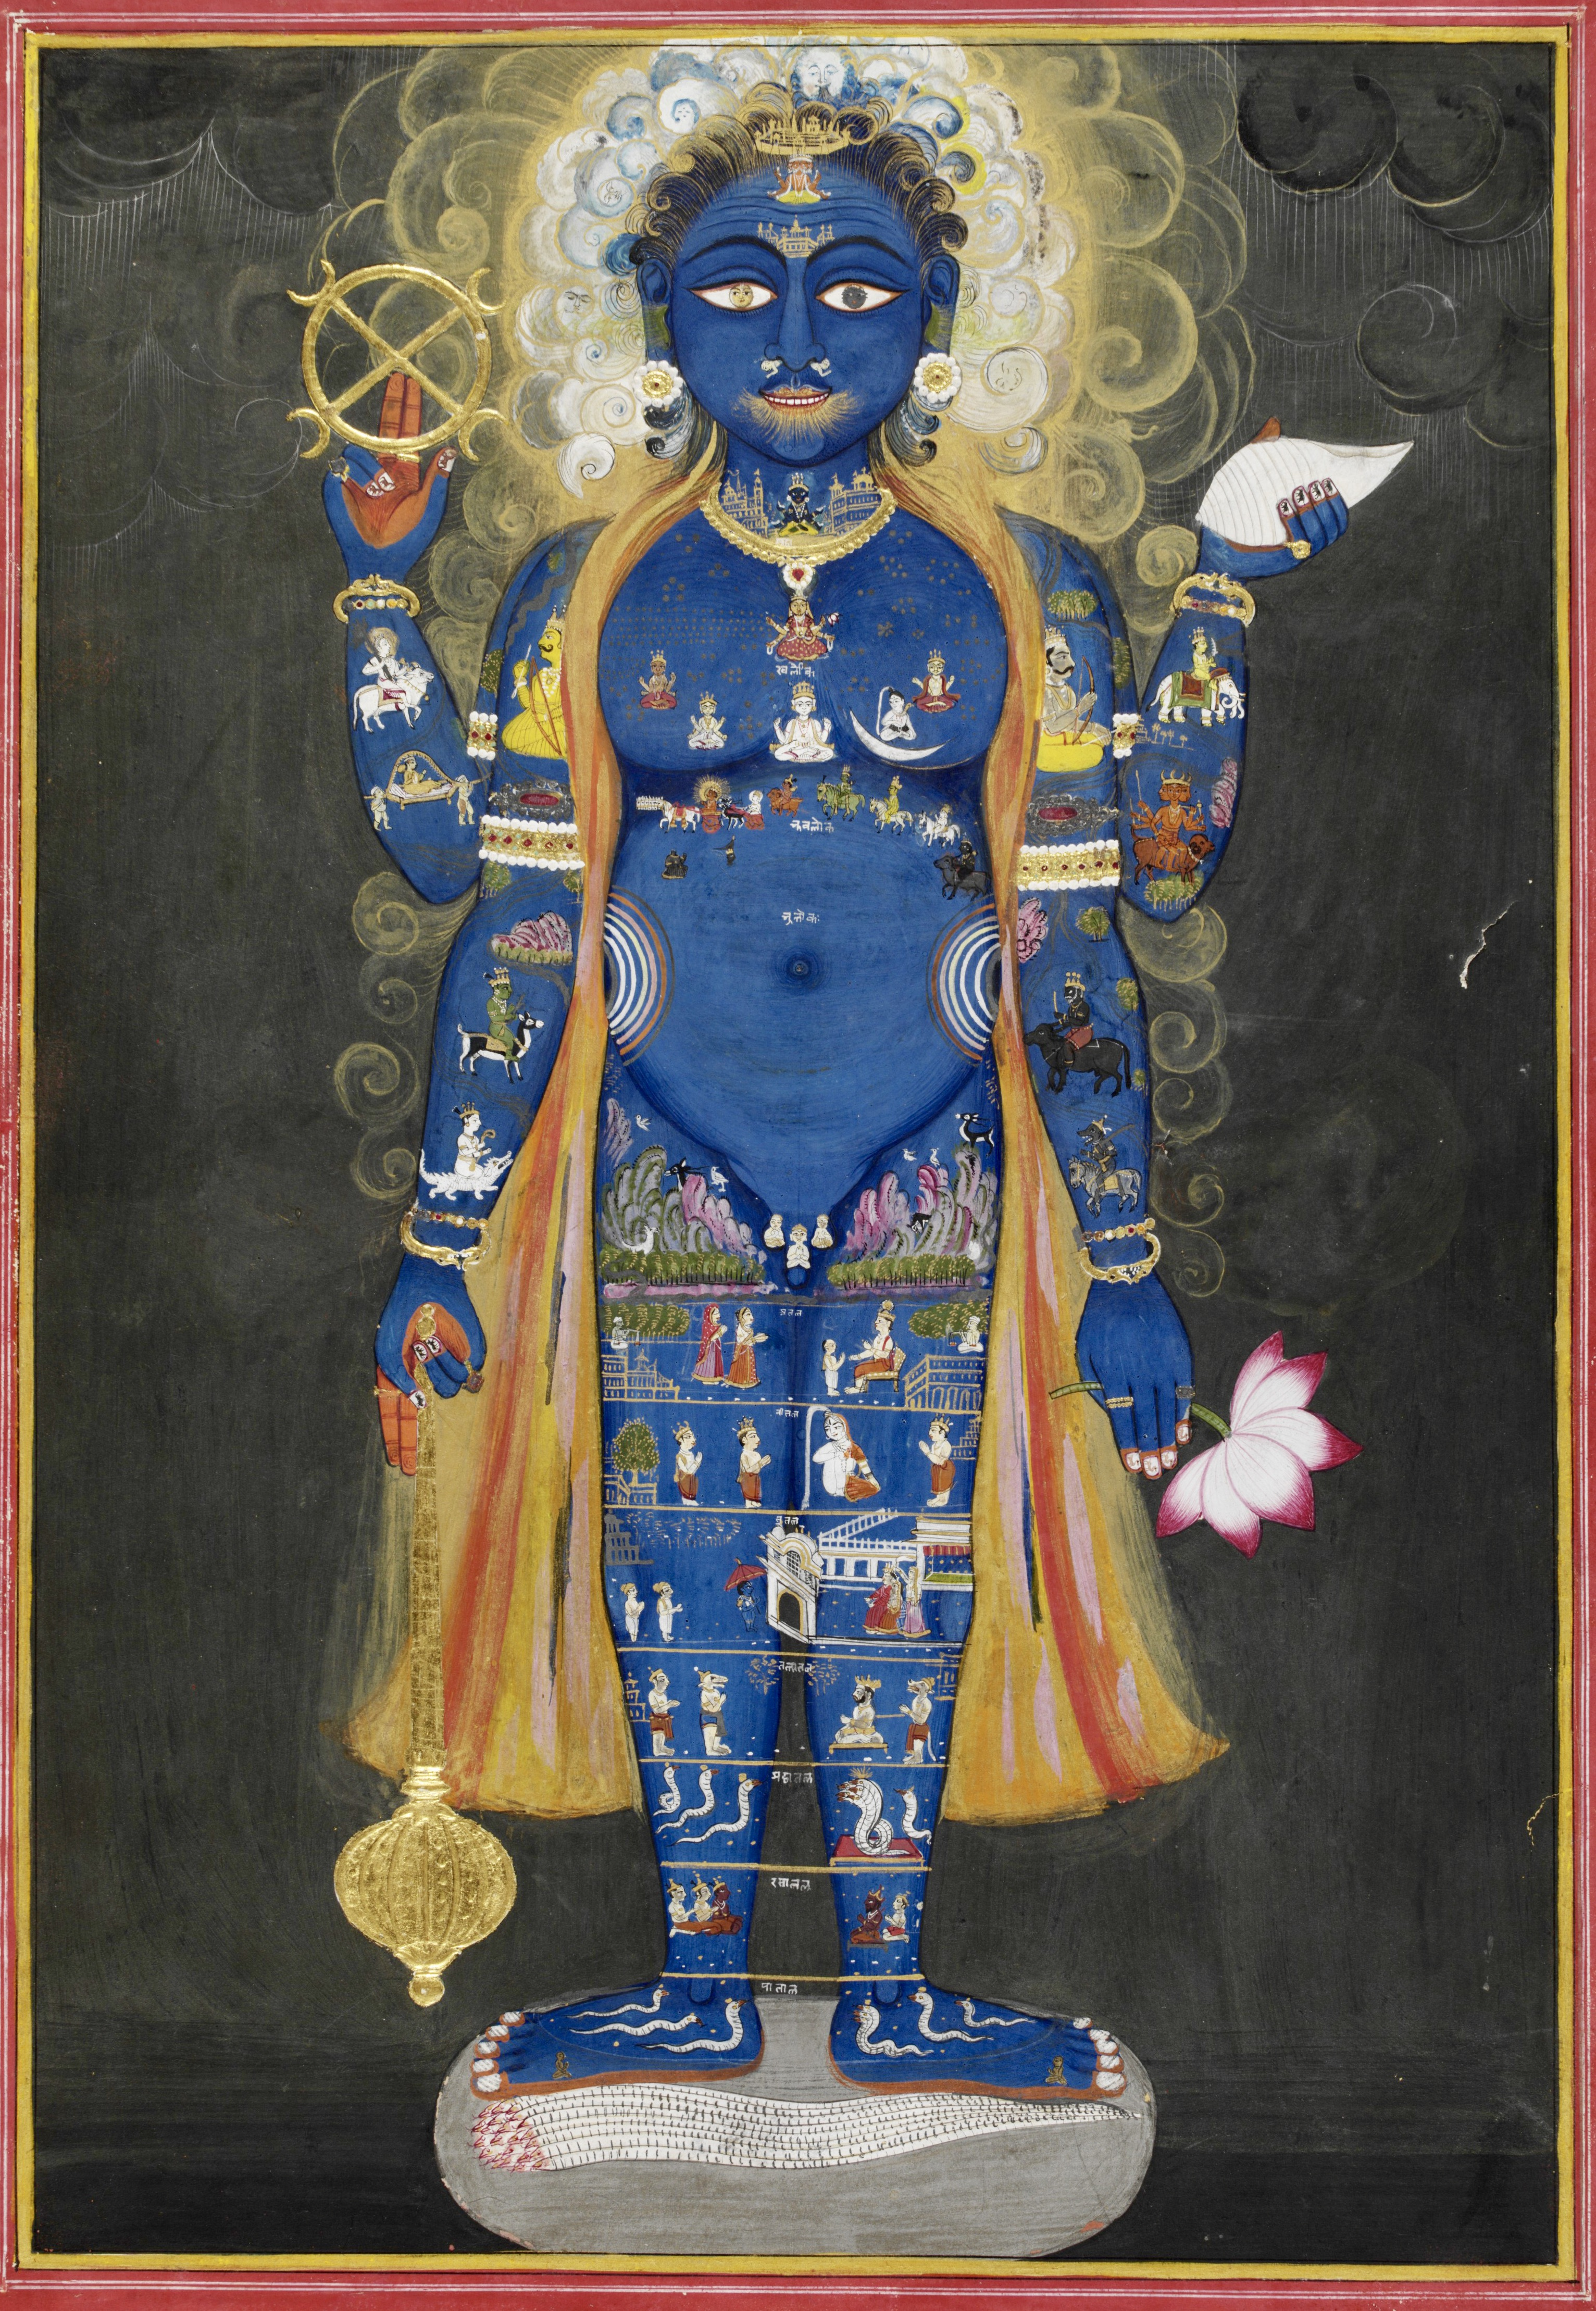
\includegraphics[width=1\textwidth]{pics/Vishnu_Vishvarupa_cropped.jpg}
	\caption{Viṣṇu Viśvarūpa, India, Rajasthan, Jaipur, ca. 1800–1820, Opaque watercolor and gold on paper, 38.5 × 28 cm, Victoria and Albert Museum, London, Given by Mrs. Gerald Clark.}
	\label{fig1}
      \end{figure}
\clearpage
  \begin{figure}[ht]
	\centering
  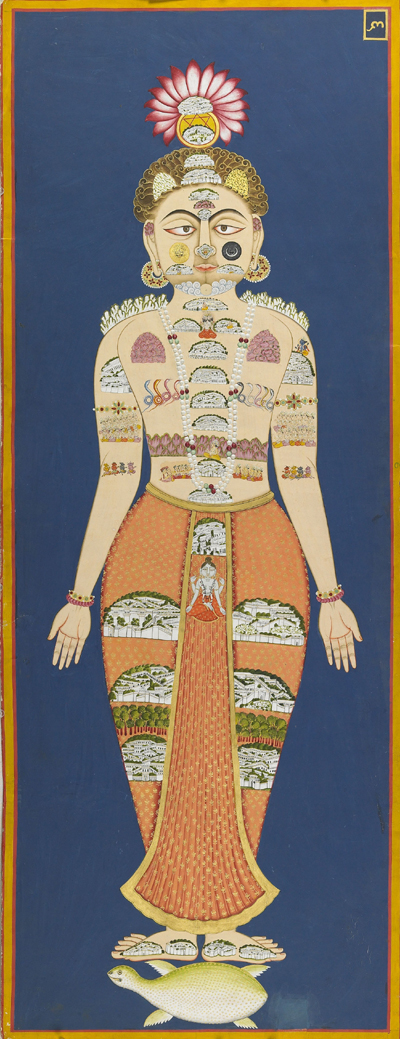
\includegraphics[width=0.5\textwidth]{pics/The_Equivalence_of_Self_and_Universe_(detail),_folio_6_from_the_Siddha_Siddhanta_Paddhati,_(Bulaki),_1824_(Samvat_1881);_122_x_46_cm._Mehrangarh_Museum_Trust..jpg}
	\caption{The Equivalence of Self and Universe (detail), folio 6 from the \textit{Siddhasiddhāntapaddhati} (Bulaki), India, Rajasthan, Jodhpur, 1824 (Samvat 1881), 122 x 46 cm, RJS 2378, Mehragarh Museum Trust.}
	\label{fig2}
      \end{figure}
      % \end{landscape}


\chapter{Bibliography}
 \label{sec:bibli}
   \clearpage
\newpage 
\thispagestyle{empty}
\quad  \addtocounter{page}{-1}

\printbibliography[heading=subbibintoc, title=Consulted Manuscripts, keyword=codex]

\printbibliography[heading=subbibintoc, title=Printed Editions, keyword=printsource]

\printbibliography[heading=subbibintoc, title=Secondary Literature, keyword=seclit]

\printbibliography[heading=subbibintoc, title=Online Sources, keyword=onlinesource]

\end{document}
